\chapter{Formale Angaben}\label{formale-angaben}

\section{Kurzüberblick über die Struktur der
Hochschule}\label{kurzuxfcberblick-uxfcber-die-struktur-der-hochschule}

\subsection{Profil der Hochschule}\label{profil-der-hochschule}

Die TH Köln ist die größte Hochschule für angewandte Wissenschaften in
Deutschland. Sie betreibt mehrere Standorte in Köln und unterhält
jeweils einen eigenen Campus in Leverkusen und Gummersbach. Aufgrund
ihrer Größe, der Angebotsvielfalt, ihres Forschungsvolumens und ihrer
internationalen Ausrichtung versteht sich als Hochschule neuen Typs mit
ausgeprägtem Praxisbezug und anwendungsorientierter Forschung.

Die TH Köln gehört der UAS7 an, dem Verbund von sieben leistungsfähigen
Fachhochschulen in Deutschland. Sie ist zudem Vollmitglied in der
European University Association (EUA). Auch Corporate Social
Responsibility ist für die Hochschule kein Fremdwort: sie ist als
familiengerechte Hochschule zertifiziert und eine nach den europäischen
öko-Managementrichtlinien EMAS und ISO 14001 geprüfte umweltorientierte
Einrichtung.

Die TH Köln pflegt eine Lehr- und Lernkultur, welche die zunehmende
Vielfalt der Studierenden in den Blick nimmt und dazu beiträgt, die
Potenziale aller Hochschulangehörigen in den Lernprozess zu integrieren
und dabei zu erschließen. Unter dem Begriff „Gute Lehre`` hat die TH
Köln einen Perspektivwechsel vom Lehrenden zum Lernenden vollzogen. Das
ganze Studium hindurch werden Studierende über Mentoring-, Tutoring- und
Blended Learning-Programme begleitet. Flexiblere Studiengangsmodelle und
hochschuldidaktische Coaching-Angebote gehören ebenso zum Portfolio wie
die Förderung leistungsstarker und sozial engagierter Studierender --
vor allem durch die Beteiligung am Deutschlandstipendium.

Ihre Programme zur hochschuldidaktischen Differenzierung, ihre
Diversity-Konzepte\footnote{https://www.th-koeln.de/hochschule/educational-diversity\_5710.php}
und ihr Programm ProfiL2\footnote{https://www.th-koeln.de/hochschule/profil\_5676.php}
für projektorientiertes Lehren und Lernen zählen zu den herausragenden
Lehr- und Lernkonzepten in Deutschland. Mithilfe eines systematischen
Qualitätsmanagements entwickelt die TH Köln die Kompetenzen in den
Bereichen Studium und Lehre, Struktur- und Curriculumentwicklung sowie
Hochschuldidaktik permanent weiter.

Die hohe Studierendenzufriedenheit und die breite Anerkennung der
Qualität eines an der TH Köln erworbenen Abschlusses sind das Fundament,
auf dem das Weiterbildungsportfolio der Hochschule aufbaut. Mit
unterschiedlichen Programmen vom Tagesseminar bis hin zum
Weiterbildungsstudium ermöglicht sie Wissenserwerb als
lebensbegleitendes Lernen. Die TH Köln versteht sich als
forschungsorientierte Hochschule für angewandte Wissenschaften. Die
Hochschule achtet bei der Auswahl des wissenschaftlichen Personals
besonders auf die berufliche Reputation und das ausgeprägte
Forschungsinteresse ihrer Lehrenden; sie fördert gezielt
Forschungsaktivitäten mit inter- bzw. transdisziplinärem Charakter. Mit
diesem innovativen Ansatz möchte sie wichtige und zukunftsweisende
Impulse zur gesellschaftlichen Entwicklung setzen. Die TH Köln arbeitet
in der Forschung deshalb intensiv mit der Wirtschaft,
Non-Profit-Organisationen, öffentlichen Einrichtungen und Verbänden,
sowie mit anderen nationalen und internationalen Hochschulen und
Wissenschaftseinrichtungen zusammen.

Die Forschungsaktivitäten beschränken sich nicht alleine auf die
Kompetenzen der Professorinnen, Professoren und wissenschaftlichen
Mitarbeiterinnen und Mitarbeiter. Vor allem über die Masterstudiengänge
bringen auch die Studierenden Kompetenzen und Kreativität in die
Forschungsprojekte ein. Um dem akademischen Nachwuchs eine weitere
wissenschaftliche Karriere zu ermöglichen, bietet die TH Köln verstärkt
kooperative Promotionen mit Universitäten an. Als aktives Mitglied der
InnovationsAllianz der nordrhein-westfälischen Hochschulen sowie der
Patentverwertungsgesellschaft PROvendis engagiert sich die Hochschule
beim Wissenstransfer zwischen Hochschulen, Wirtschaft und Gesellschaft.

Auch international pflegt die TH Köln enge Beziehungen zu anderen
Hochschulen. Sie ist derzeit Partnerin von rund 290 Hochschulen im
Ausland und unterstützt über ein breites Angebot von
Auslandsaufenthalten und Fördermöglichkeiten die Mobilität der
Studierenden. So werden mehrere Masterstudiengänge komplett in
englischer Sprache angeboten. Ein Drittel der Studierenden aus dem
Ausland kommt aus Übersee: aus Afrika, Amerika, Asien oder Australien.

\subsection{Lehr- und
Forschungsschwerpunkte}\label{lehr--und-forschungsschwerpunkte}

Die TH Köln ist eine forschungsaktive und forschungsstarke Hochschule.
Sie kooperiert national und international mit Universitäten und anderen
Forschungseinrichtungen, da hochwertige Forschung vom fachlichen
Austausch lebt -- über institutionelle und geographische Grenzen hinweg.

Klimawandel, knappe Ressourcen, Sicherheit und demographischer Wandel
sind einige der großen Herausforderungen der nächsten Jahrzehnte. Die
erfahrenen Wissenschaftlerinnen und Wissenschaftler der TH Köln forschen
im Rahmen ihrer anwendungsorientierten und interdisziplinären Projekte
an Lösungen für diese „Great Challenges`` und leisten einen aktiven
Beitrag zur Weiterentwicklung von Wissenschaft, Wirtschaft und
Gesellschaft.

Die vielfältigen Forschungsaktivitäten spiegeln sich im Forschungsprofil
der TH Köln, bestehend aus 10 thematischen Clustern\footnote{https://www.th-koeln.de/forschung/cluster\_2734.php}
wider. Die Cluster dienen als thematische Klammer für die
Forschungsaktivitäten in den unterschiedlichen Forschungsstrukturen der
Hochschule, wie Forschungsinstitute, Kompetenzplattformen,
Forschungsschwerpunkten und Forschungsstellen.

\subsection{Zahl und Verteilung der
Studierenden}\label{zahl-und-verteilung-der-studierenden}

An der TH Köln studieren ca. 23.500 Studierende an 11 Fakultäten. Die
Abbildung\footnote{Abbildung Verteilung der Studierenden} zeigt die
Verteilung der Studierenden.

\section{Einbettung der Studiengänge in die
Fakultät}\label{einbettung-der-studienguxe4nge-in-die-fakultuxe4t}

Die Fakultät für Informatik und Ingenieurwissenschaften ist am Standort
Gummersbach angesiedelt (Campus Gummersbach) und ist mit derzeit 5200
Studierenden\footnote{Studentenzahlen\_WS-2016\_(01.12.2016).pdf} die
größte Fakultät der TH Köln. An der Fakultät sind 8 Institute
angesiedelt; zum Studienangebot der Fakultät gehören 8 Bachelor- und 6
Masterstudiengänge. Die Medieninformatik Studiengänge werden von der
Fakultät für Informatik und Ingenieurwissenschaften ausgerichtet und ist
im Institut für Informatik organisatorisch verankert.

Das Institut für Informatik betreibt Labore für: - Allgemeine
Datenverarbeitung (ADV) - Systemgestaltung (SG) - Mathematik \& ihre
Anwendungen - Medieninformatik (MI) - Mobile und verteilte
Informationstechnologie (moxd) - Kommunikationstechnik \&
Datensicherheit (KTDS) - Wirtschaftsinformatik (WI)

\begin{verbatim}
    Aktueller Bearbeiter: -
    Bearbeiterhistorie: Christian Noss
    Date: 14.02.2017
    Comment: Inhaltlich ok, Abbildung Verteilung der Studierenden fehlt.
    Status: Peer-Review erforderlich
    Reviewed von: -
\end{verbatim}

Die Studiengänge wurden auf Basis verschiedener quantitativer und
qualitativer Erhebungen analysiert und in einem iterativen Prozess
optimiert. An diesem Prozess waren folgende Personengruppen beteiligt:

\begin{longtable}[]{@{}ll@{}}
\toprule
\begin{minipage}[b]{0.5\columnwidth}\raggedright\strut
Beteiligte Personengruppe\strut
\end{minipage} & \begin{minipage}[b]{0.5\columnwidth}\raggedright\strut
Art der Beteiligung\strut
\end{minipage}\tabularnewline
\midrule
\endhead
\begin{minipage}[t]{0.5\columnwidth}\raggedright\strut
Professoren der Medieninformatik-spezifischen Module\strut
\end{minipage} & \begin{minipage}[t]{0.5\columnwidth}\raggedright\strut
regelmäßige Akkreditierungstreffen\strut
\end{minipage}\tabularnewline
\begin{minipage}[t]{0.5\columnwidth}\raggedright\strut
Professoren der Medieninformatik-übergreifenen Module\strut
\end{minipage} & \begin{minipage}[t]{0.5\columnwidth}\raggedright\strut
themenspezifische Abstimmungsmeetings, Einzelgespräche\strut
\end{minipage}\tabularnewline
\begin{minipage}[t]{0.5\columnwidth}\raggedright\strut
Studierende\strut
\end{minipage} & \begin{minipage}[t]{0.5\columnwidth}\raggedright\strut
Evaluationen, Einzelgespräche, Feedbackrunden\strut
\end{minipage}\tabularnewline
\begin{minipage}[t]{0.5\columnwidth}\raggedright\strut
wissenschaftliche Mitarbeiter der Medieninformatik\strut
\end{minipage} & \begin{minipage}[t]{0.5\columnwidth}\raggedright\strut
Einzelgespräche, Feedbackrunden\strut
\end{minipage}\tabularnewline
\begin{minipage}[t]{0.5\columnwidth}\raggedright\strut
Prüfungsausschuss\strut
\end{minipage} & \begin{minipage}[t]{0.5\columnwidth}\raggedright\strut
themenspezifische Abstimmungsmeetings, Einzelgespräche\strut
\end{minipage}\tabularnewline
\begin{minipage}[t]{0.5\columnwidth}\raggedright\strut
Prüfungsamt\strut
\end{minipage} & \begin{minipage}[t]{0.5\columnwidth}\raggedright\strut
themenspezifischen Abstimmungsmeetings, Einzelgespräche\strut
\end{minipage}\tabularnewline
\begin{minipage}[t]{0.5\columnwidth}\raggedright\strut
Qualitätsmanagement-Team\strut
\end{minipage} & \begin{minipage}[t]{0.5\columnwidth}\raggedright\strut
themenspezifische Abstimmungsmeetings, Einzelgespräche\strut
\end{minipage}\tabularnewline
\begin{minipage}[t]{0.5\columnwidth}\raggedright\strut
Alumni und Wirtschaftsvertreter\strut
\end{minipage} & \begin{minipage}[t]{0.5\columnwidth}\raggedright\strut
Evaluationen, Einzelgespräche\strut
\end{minipage}\tabularnewline
\bottomrule
\end{longtable}

\begin{verbatim}
    Aktueller Bearbeiter: Christian Noss
    Bearbeiterhistorie: Christian Noss
    Date: 14.02.2017
    Comment: erstmal fertig
    Status: Peer-Review erforderlich
    Reviewed von: -
\end{verbatim}

\chapter{Ist-Zustand}\label{ist-zustand}

\section{Erfüllung der Auflagen der Reakkreditierung
2010}\label{erfuxfcllung-der-auflagen-der-reakkreditierung-2010}

Der Technischen Hochschule Köln wurden im Rahmen der Reakkreditierung im
März 2010 folgende Auflagen der Akkreditierungskommission mitgeteilt.

\subsection{Auflagen Medieninformatik
Bachelor}\label{auflagen-medieninformatik-bachelor}

\begin{quote}
\begin{enumerate}
\def\labelenumi{\arabic{enumi}.}
\tightlist
\item
  Die Prüfungsorganisation muss gewährleisten, dass
  studienzeitverlängernde Effekte beim Übergang vom Grund- zum
  Hauptstudium vermieden werden.
\item
  Eine Beschreibung des Moduls Abschlussarbeit muss erstellt werden.
\end{enumerate}
\end{quote}

Die Auflagen für den Bachelor-Studiengang Medieninformatik wurden von
der Fachhochschule Köln folgendermaßen erfüllt:

\begin{itemize}
\tightlist
\item
  zu 1: In §17 (3) der Bachelorprüfungsordnung wurde der folgende Passus
  ersatzlos gestrichen: Zu den Modulprüfungen des Hauptstudiums (Teil
  1), mit Ausnahme des Moduls ``Netzbasierte Anwendungen'', wird
  zugelassen, wer die Zwischenprüfung mit einer beliebigen Ausnahme
  bestanden hat. Zu den Modulprüfungen des Hauptstudiums (Teil 2) wird
  zugelassen, wer die Zwischenprüfung ohne Ausnahme bestanden hat. Somit
  gibt es keine der Prüfungsorganisation anzulastenden
  studienzeitverlängernden Effekte beim Übergang vom Grund- zum
  Hauptstudium mehr.
\item
  zu 2: Die Beschreibung des Moduls Abschlussarbeit wurde vorgelegt.
\end{itemize}

\subsection{Auflagen Medieninformatik
Master}\label{auflagen-medieninformatik-master}

\begin{quote}
\begin{enumerate}
\def\labelenumi{\arabic{enumi}.}
\tightlist
\item
  Es muss sichergestellt werden, dass den Studierenden zu Beginn der
  Veranstaltungen die Form der Prüfungsleistungen bekannt gegeben wird
  und diese auf die Ausbildungsziele abgestimmt ist.
\item
  Vorlage der gemäß den Auflagen geänderten und in Kraft gesetzten
  Ordnungen.
\end{enumerate}
\end{quote}

Diese Auflagen wurden von der Technischen Hochschule Köln folgendermaßen
erfüllt:

\begin{itemize}
\tightlist
\item
  zu 1: Nach unserer Auffassung entspricht die vorgelegte Klausel der
  von der Agentur gewünschten Regelung. Insbesondere ist in §16(4) der
  Prüfungsordnung festgelegt: ``Der Prüfungsausschuss legt in der Regel
  zu Beginn eines Semesters im Benehmen mit den Prüferinnen und Prüfern
  für jedes Modul die Prüfungsform und die Prüfungsmodalitäten \ldots{}
  fest.'' Die von der Agentur angemerkte Zweimonatsfrist bezieht sich
  nur auf die Festlegung des Prüfungszeitraums - nicht auf die Form. Zu
  Semesteranfang bedeutet nach unserer Auffassung 1. April oder 1.
  September des Jahres, also ca. 1 Monat vor Veranstaltungsbeginn. Die
  Flexibilität durch den Passus ``in der Regel'' sollte erhalten
  bleiben, um bspw. auf Erkrankungen oder Ausfall von Dozenten, bzw.
  Lehrbeauftragten oder andere, von außen einwirkende Ereignisse
  reagieren zu können. Die seitens der Studierenden geäußerte Kritik
  hinsichtlich der betreffenden Fristen interpretieren wir so, dass die
  Regelung vermutlich in Ausnahmefällen von einzelnen Dozenten nicht
  vollständig umgesetzt wurde. Von daher erscheint es uns angeraten,
  eine eigentlich in sich konsistente Prüfungsordnung an dieser Stelle
  nicht zu ändern, sondern die Umsetzung zu verbessern. Dazu wird die
  folgende explizite und zentralisierte Verfahrensweise zur
  verbindlichen Bekanntgabe der Prüfungsform zu Beginn des Semesters
  festgelegt:
\item
  Falls die Prüfungsform dem im Internet oder beim
  Studiengangsbeauftragten einsehbaren Modulhandbuch entspricht, gilt
  diese damit als bekannt gemacht. Diese Teilregelung wird dauerhaft im
  Prüfungsamt ausgehängt.
\item
  Sollte die Prüfungsform, bspw. wegen aktueller didaktischer
  Erwägungen, von der im Modulhandbuch bekannt gemachten Form abweichen,
  so ist diese durch den Dozenten dem Prüfungsamt rechtzeitig
  mitzuteilen, welches über die Änderung dann per Aushang fristgerecht
  informiert. § 14 der Prüfungsordnung für den Masterstudiengang
  Medieninformatik wurde dementsprechend neu gefasst.
\item
  zu 2: Die Prüfungsordnungen vom 7. Januar 2011, in denen alle Auflagen
  erfüllt sind, wurden vom Fakultätsrat der Fakultät für Informatik und
  Ingenieurwissenschaften am 10.11.2010 bzw. 6.1.2011 beschlossen und
  vom Präsidenten der Fachhochschule Köln am 7.1.2011 genehmigt. Sie
  liegen der ASIIN vor.
\end{itemize}

\section{Stärken und Schwächen
Analyse}\label{stuxe4rken-und-schwuxe4chen-analyse}

\subsection{Beurteilung des Studienerfolgs auf der Basis von
Absolventenbefragungen und
Verbleibstudien}\label{beurteilung-des-studienerfolgs-auf-der-basis-von-absolventenbefragungen-und-verbleibstudien}

Die folgenden Ausführungen beruhen auf der Datenerhebung\footnote{Statistik
  zum Verbleib- und Studienabbruch} zum 01.12.2015 für den Zeitraum 2011
bis 2015 und fokussieren die derzeit eingeschriebenen Studierenden,
erfolgreiche Abschlüsse und Studienfachabbrecher im
Medieninformatik-Bachelor.

\begin{verbatim}
cn: Tabelle zeigt nur Zahlen bis 2013. Haben wir da was besseres?
\end{verbatim}

\{\% include image.html url=``tabellen/MI-BA-anzahl-studierende.svg''
caption=``Tabelle 1: Daten des Bachelorstudiengangs Medieninformatik''
\%\}

Die in Tabelle 1 dargestellten Zahlen zeigen einen stetig wachsenden
Zulauf für den Bachelorstudiengang Medieninformatik, der ursprünglich
für 63 Studierende ausgelegt wurde. Erfreulicherweise ist, trotz der im
Rahmen der Fakultätsentwicklung und des Hochschulentwicklungsplans
2020\footnote{Hochschulentwicklungsplan 2020} steigenden Anfängerzahlen,
eine gleichbleibende Abbrecherquote um die 30\% zu erkennen. Die Zahlen
zeigen leider auch eine niedrige Quote an Absolventen in
Regelstudienzeit, die jedoch im Mittel aller Studiengänge der Fakultät
10 liegt. Nach den vorliegenden Prüfungsstatistiken (vgl.
Prüfungsstatistiken \footnote{Bachelorstudiengang Medieninformatik,
  Prüfungsstatistik 2016}) ist mit einem proportionalen Anstieg der
Absolventen zu rechnen.

\begin{verbatim}
@Volker: kann die Tabellennummerierung automatisiert werden?
\end{verbatim}

Die im Rahmen der letzten Reakkreditierung eingebrachten Änderungen
können hinsichtlich der Quote der Studienabbrecher bereits als recht
erfolgreich bewertet werden. Vor allem die Auflösung der strikten, durch
Zulassungsvoraussetzungen in der Prüfungsordnung verankerte Trennung von
Grund- und Hauptstudium hat die Dauer des Fachstudiums definitiv
verkürzt. Auch die Einführung des Moduls „Einführung in die
Medieninformatik`` (EMI) erweist sich als sinnvoll und notwendig, um den
Studierenden früh die Perspektiven und fachlichen Aspekte der
Medieninformatik näher zu bringen.

Aus der INCHER-Studie von 2014\footnote{INCHER-Studie 2014} geht für
alle Studiengänge in NRW hervor: wer während des Studiums ein
Firmenpraktikum absolviert, schließt das Studium etwas seltener in der
Regelstudienzeit ab (54 Prozent vs.~60 Prozent). Ähnlich ist die Tendenz
ist zwischen denjenigen, die ihr Studium hauptsächlich durch
Erwerbsarbeit finanzierten und den übrigen Absolventinnen und
Absolventen zu erkennen: Wenn das Studium durch eigene Erwerbsarbeit
finanziert wurde, wird es ebenfalls seltener in der Regelstudienzeit
abgeschlossen (50 Prozent vs.~57 Prozent).

Schlussfolgerungen über die Studienqualität sind auf Grundlage der
verfügbaren Daten nur bedingt möglich. Als Ausgangspunkt für die, im
Rahmen der Reakkreditierung zu anzustrebenden Änderungen, wurden daher
zusätzlich folgende Quellen mit einbezogen:

\begin{itemize}
\tightlist
\item
  Studentische Rückmeldungen aus den, im Rahmen des Medieninformatik
  Showcase stattfindenden Feedbackrunden
\item
  Persönliche Gespräche mit Studierenden, Alumni und
  Kooperationspartnern
\item
  Probleme und Fragen, die an die Medieninformatik Mentorin und die
  Studiengangsmanager gerichtet wurden
\item
  Befragung der beteiligten Professoren, wissenschaftlichen Mitarbeitern
  und Tutoren
\item
  Rückschlüsse aus Veranstaltungsevaluationen
\item
  Gespräche mit Unternehmensvertretern
\end{itemize}

Auf dieser Basis konnten, bezogen auf die bereits beschrieben
Erkenntnisse der INCHER-Studie, zwei Gründe für verlängerte Studiendauer
ermittelt werden:

\begin{itemize}
\tightlist
\item
  Viele Studierende finanzieren ihr Studium, vor allem in höheren
  Semestern und im Master-Studium, durch Erwerbsarbeit.
\item
  Das große Modul ``Entwicklungsprojekt interaktive Systeme'' (10
  Creditpoints) überfordert viele Studierende.
\item
  Das Praxisprojekt im sechsten Semester wird in der Regel in
  Kooperation mit Unternehmen absolviert.
\end{itemize}

Bei den Vorbereitungen zum Praxisprojekt, das in der Regel im selben
Themenfeld wie die Bachelorarbeit absolviert wird, durchlaufen die
Studierenden in der Regel einen dreistufigen Prozess:

\begin{enumerate}
\def\labelenumi{\arabic{enumi}.}
\tightlist
\item
  Identifikation eines geeigneten Themenfeldes für das Praxisprojext, in
  der Regel in Absprache mit einem oder mehreren Dozenten.
\item
  Bewerbung bei passenden Kooperationspartnern in der Wirtschaft.
\item
  Einarbeitung beim Unternehmen und Einigung auf das finale Thema zum
  Praxisprojekt mit dem Unternehmen und dem Dozenten.
\end{enumerate}

Dieser Prozess ist zeitaufwändig und wird von den meisten Studierenden
unterschätzt und daher häufig zu spät begonnen. Um diesem Problem
entgegen zu wirken wird in der Medieninformatik seit drei Jahren am Ende
des fünften Semesterseine Kontaktbörse durchgeführt. Auf dieser
Veranstaltung werden den künftigen Absolventen die Regularien, Abläufe
und Herausforderungen des Abschlusssemesters erläutert. Darüber hinaus
stellen ausgewählte Unternehmen und Organisationen potenzielle Themen
und Problemfelder für Praxisprojekt und Bachelorarbeit vor. Auch die
Professoren der Informatik haben hier die Möglichkeit ihre Themen und
Forschungsfelder als Ansatzpunkt für mögliche, forschungsnahe
Praxisprojekte und Abschlussarbeiten vorzustellen.

\subsection{Bewertung von Ergebnissen der
Evaluation}\label{bewertung-von-ergebnissen-der-evaluation}

Hier kann auf Erstsemesterbefragungen und regelmäßig semesterweise
durchgeführte Evaluationen der Lehrveranstaltungen verwiesen werden. Die
Auswertung der Evaluationen erfolgt zentral durch die
Hochschulverwaltung; ein integriertes Qualitätsmanagement nach DIN/ISO
9001 ist an der Fakultät 10 etabliert. In den Ergebnissen\footnote{Studentische
  Evaluationen Medieninformatik} zeigt sich grundsätzlich bei den
Bachelorstudierenden ein etwas geringeres Zufriedenheitsmaß als bei den
Masterstudierenden. Dies lässt sich mit Verweis auf die allgemein hohen
Abbruchquoten in grundständigen Informatikstudiengängen ggf. so
interpretieren, dass die Unzufriedenheit nicht allein durch die
Studienangebotsseite verursacht ist. Dennoch lassen sich deutliche
Verbesserungspotentiale identifizieren, etwa bzgl. der Einführung neuer
Lehr-Lernformate, Koordination der Praktika, Bereitstellung von
studentischen Arbeitsräumen, Gastvorträgen, Exkursionen und Workshops.

Der 2013 zu verzeichnende Rückgang der Zufriedenheit bzgl. des
Lehrangebotes im Master lässt sich nach unseren Analysen und Gesprächen
mit Studierenden u.A. als Auswirkung des ersten, im Informatik-Master
durchgeführten Projekt-Semesters interpretieren. Die dort durchgeführten
„Guided Projects`` zeigen einen starken Praxisbezug und eine klare, mit
den Methoden des (oft agilen) Projektmanagements gestaltete
Ablaufstruktur.

\begin{verbatim}
cn: hier fehlt noch die explizite Schlussfolgerung
\end{verbatim}

Die Unzufriedenheit bei der Bewertung der Studien- und
Prüfungsorganisation in der Fakultät lässt sich auf punktuelle Ausfälle
des ``Prüfungs- und Studierendenservice Online'' (PSSO) und teilweise
nicht optimal im Internet kommunizierte Prüfungsinformationen
zurückführen. Erfreulich ist die weiterhin große Gesamtzufriedenheit der
Studierenden im Medieninformatik Master.

\subsection{Außercurriculare
Maßnahmen}\label{auuxdfercurriculare-mauxdfnahmen}

Mehrere gebündelte und ständig weiter entwickelte außercurriculare
Maßnahmen tragen, insbesondere vor dem Hintergrund der stark
ansteigenden Studierendenzahlen, zur weiteren Verbesserung der
Studienqualität bei.

\paragraph{Showcase}\label{showcase}

Das jährlich durchgeführte Medieninformatik-Showcase dient zur Stärkung
der Identität der Medieninformatik, zur besseren Vernetzung von
Studierenden sowohl zwischen Master- und Bachelorstudierenden als auch
über die Studiensemester, zum Ausblick auf die Praxis durch externe
Sprecher (oft Alumni), sowie als strukturierte Feedbackmöglichkeit. Das
Event verbessert außerdem die Sichtbarkeit der Medieninformatik am
Campus und in der Region.

\paragraph{Medieninformatik Mentor}\label{medieninformatik-mentor}

Der neu eingeführte Medieninformatik Mentor, welcher mit erfahrenen
wissenschaftlichen Mitarbeiterinnen oder Mitarbeitern besetzt wird, die
selbst zumindest den Bachelorstudiengang Medieninformatik am Campus
Gummersbach absolviert haben, um mit den Studierenden Probleme im und um
das Studium zu besprechen und als institutionelles Bindeglied zwischen
Studierenden und Lehrenden fungiert.

\paragraph{Social Media Angebote}\label{social-media-angebote}

Die von der Medieninformatik eingerichteten und administrierten Social
Media Angebote in YouTube, Facebook- und Twitter erreichen regelmäßig
etwa 1000 Abonnenten, sprich: Studierende, Interessierte und Alumni. Sie
bieten eine gute Gelegenheit um im Gespräch zu bleiben, Themen und
Arbeitsergebnisse zu platzieren, sowie Studienanfänger, Jobs und
Projekte zu akquirieren oder anzubieten.

\paragraph{\texorpdfstring{Wettbewerb ``Die besten
Projekte''}{Wettbewerb Die besten Projekte}}\label{wettbewerb-die-besten-projekte}

Der jährlich vom Labor für Medieninformatik durchgeführte Wettbewerb
``Die besten Projekte'', welcher einerseits gute und sehr gute
Ergebnisse aus dem Bachelor- und dem Masterstudiengang herausstellt,
andererseits in der gemeinsamen Abschlusspräsentation zur Vernetzung
zwischen den Studierenden des Bachelor- und des Masterstudiengangs
beiträgt, und letztendlich den projektorientierten Ansatz in der
Medieninformatik nachhaltig sichtbar macht.

\paragraph{Medieninformatik
Kontaktbörse}\label{medieninformatik-kontaktbuxf6rse}

Die bereits beschriebe, einmal im Semester durchgeführte,
Medieninformatik Kontaktbörse dient zur Erleichterung des Übergangs in
das Abschlusssemester, zur Herstellung von Kontakten zu potentiellen
Kooperationspartnern, und zum Geben von Ideen und Inspiration zu Themen
für die Abschlussarbeit.

\paragraph{Medieninformatik-Filmfest}\label{medieninformatik-filmfest}

Das jährlich durchgeführte Medieninformatik-Filmfest dient zur Stärkung
der Identität der Medieninformatik, zur besseren Vernetzung der
Studierenden, insbesondere der Studienanfänger und zur Präsentation
ausgewählter Arbeitsergebnisse. Das Event verbessert außerdem die
Sichtbarkeit der Medieninformatik am Campus und in der Region.

\subsection{Bewertung der statistischen Daten bezüglich der
Auslastung, der Prüfungserfolge, der Abbrecherquoten und der
Studienanfängerund
Bewerberzahlen.}\label{bewertung-der-statistischen-daten-bezuxfcglich-der-auslastung-der-pruxfcfungserfolge-der-abbrecherquoten-und-der-studienanfuxe4ngerund-bewerberzahlen.}

Die folgenden Ausführungen beruhen auf der Datenerhebung zum 22.09.2016
für den Zeitraum Wintersemester 2011 bis Wintersemester 2015\footnote{Bachelorstudiengang
  Medieninformatik, Prüfungsstatistik 2016}\footnote{Fakultät für
  Informatik und Ingenieurwissenschaften, Statistik 2013/14} und
fokussieren die derzeit eingeschriebenen Studenten, erfolgreiche
Abschlüsse und Studienfachabbrecher.

Zur Bewertung der Auslastung kann wie folgt Stellung genommen werden:
gemessen an den planmäßigen 63 Studierendenplätzen (WS13/14) werden seit
drei Studienjahren im Rahmen der strategischen Fakultätsplanung und des
Hochschulentwicklungsplans 2020 mehr als 200\% Überlast aufgenommen. Mit
den Abbrecherquoten im Bachelorstudiengang bewegt sich die
Medieninformatik im breiten Mittelfeld von Informatikstudiengängen im
Allgemeinen; \textsubscript{\textasciitilde{}} cn: gibt es zu ``im
breiten Mittelfeld von Informatikstudiengängen'' zahlen?
\textsubscript{\textasciitilde{}}

sehr erfreulich ist die für den Masterstudiengang Medieninformatik die
geringe Abbrecherquote. In Verbindung mit der bedauerlich hohen, für
ingenieur- und naturwissenschaftliche Studiengänge, insbesondere im
Bachelor-Bereich jedoch leider inhärenten Abbrecherquote
(durchschnittlich geschätzte Schwundquote in der Informatik an
Fachhochschulen ist 39\%), \textsubscript{\textasciitilde{}} cn: wo
kommt diese Zahl her (durchschnittlich geschätzte Schwundquote in der
Informatik an Fachhochschulen ist 39\%)?
\textsubscript{\textasciitilde{}} zeigt sich hier ein deutliches noch zu
hebendes Optimierungspotential. Erfreulich ist hier die mit 27\% recht
hohe Frauenquote im Bachelorstudiengang Medieninformatik. Die
durchschnittliche Frauenquote in der Lehreinheit Informatik liegt bei
22\%. In der Fakultät 10 liegt sie bei 20\%.

Die Prüfungserfolge sind bzgl. des Bachelor- und Masterstudiengangs zu
differenzieren.

Im Bachelorstudiengang Medieninformatik zeigt sich bei den
Prüfungserfolgen des „neuen`` im Vergleich zum „alten`` Studiengang
(BPO2 vs.~BPO3, s. Anhang Pruefungsstatistiken \footnote{Bachelorstudiengang
  Medieninformatik, Prüfungsstatistik 2016}) ein früherer
Prüfungserfolg. Auch in höheren Semestern werden die Prüfungen früher
absolviert und mit weniger Fehlversuchen bestanden. In erster Näherung
findet man den ersten beiden Semestern eine Gleichverteilung der Noten
innerhalb des Notenspektrums, die sich in den höheren Semestern zu einer
deutlichen Verbesserung hin verschiebt. Hier mögen zwei Faktoren von
Bedeutung sein: zum einen der deutlich höhere Anteil an
medien(informatik)spezifischen Modulen und zum anderen kann gemutmaßt
werden, dass sich hier die Abbrecherzahlen positiv auswirken. Die
Abschluss- und die Endnoten setzen diesen Trend der Verbesserung des
Notendurchschnitts fort.

Im Masterstudium wirkt die sich die, im Rahmen der Reakkreditierung
weggefallene Zulassungsvoraussetzung eines Mindest-Notenschnittes nicht
wesentlich auf die Verteilung der Prüfungsergebnisse aus. Auch hier ist
weiterhin das gesamte Notenspektrum abgedeckt, ebenso wie bei den
Ergebnissen der Master Thesen.

\subsection{Rückschlüsse aus informellen Gesprächen und
Kommentaren}\label{ruxfcckschluxfcsse-aus-informellen-gespruxe4chen-und-kommentaren}

\begin{itemize}
\tightlist
\item
  vertiefende Kenntnisse von verschiedenen Programmierkonzepte
\end{itemize}

\begin{verbatim}
cn: TBD
\end{verbatim}

\subsection{Ableitungen aus den Bewertungen der zur Verfügung
stehenden Daten und
Evaluationen}\label{ableitungen-aus-den-bewertungen-der-zur-verfuxfcgung-stehenden-daten-und-evaluationen}

Aus den Bewertungen der Daten, Evaluationen und Feedbacks lassen sich
folgende Stärken und Schwächen ableiten.

\paragraph{Stärken des Medieninformatik
Bachelor}\label{stuxe4rken-des-medieninformatik-bachelor}

\paragraph{Schwächen des Medieninformatik
Bachelor}\label{schwuxe4chen-des-medieninformatik-bachelor}

Als Indikator für eine gute Studierbarkeit, kann die Anzahl der
abgelegten Prüfungen im vorgesehenen Fachsemester des Moduls angesehen
werden. Ziel ist es, dass die Studierenden Prüfungen möglichst im selben
Semester ablegen, in dem das Modul im Studienverlaufsplan verortet ist.
Gelingt dies nicht, so kann ein Studienabschluss innerhalb der
Regelstudienzeit fast nicht mehr realisiert werden. Ab dem dritten
Studiensemester werden Prüfungen zunehmend verspätet abgelegt (vgl.
Pruefungsstatistiken\footnote{Bachelorstudiengang Medieninformatik,
  Prüfungsstatistik 2016}). Feedbacks, Befragungen und
Curriculumsanalyse\footnote{fehlt} zeigen, dass in diesem Semester die
Anzahl der unterschiedlichen Module am höchsten ist und viele Module
Praxisanteile in Projektform haben, so dass sich die Studierenden in
verschiedene Fachdisziplinen, Modulregularien und Projektkontexte
eindenken und vielen Teamkonstellationen organisieren müssen.
Darüberhinaus sind im dritten Semester bei vielen Modulen
Prüfungsvorleistungen (Teilnahmeschein) notwendig.

Ein weiteres Problem bildet offenbar das große Projekt im fünften
Semester (Entwicklungsprojekt interaktive Systeme). Nachdem die
Studierenden in den vorangegangen Semestern nur mit Projektgrößen von
maximal 2,5 Creditpoints konfrontiert wurden, stehen sie im fünften
Semester einem Projekt der vierfachen Größe gegenüber. Dies scheint
viele zu überfordern, so dass sie entweder erst dann das Projekt
beginnen, wenn sie keine parallelen Veranstaltungen haben, oder das
Projekt vorzeitig abbrechen.

Die Probleme beim Übergang ins Abschlusssemester wurden bereits
beschrieben. Vor allem in Feedbacks und persönlichen Gesprächen wird ein
weiteres Defizit häufig genannt: die fehlende Möglichkeit sich in einem
thematischen Bereich zu vertiefen.

\begin{verbatim}
cn: hier fehlt auch eine Schlussfolgerung
\end{verbatim}

Somit lassen sich die folgenden Defizite im aktuellen Medieninformatik
Bachelor Studiengang zusammenfassen:

\begin{itemize}
\tightlist
\item
  Überladenes drittes Fachsemester
\item
  Zu viele Projektkontexte
\item
  Zu großer Sprung der Projektgrößen
\item
  Zu viele verschiedene Module mit unterschiedlichen Regularien
\item
  Zeitproblem beim Einstieg ins Praxisprojekt
\item
  Fehlende Möglichkeit zur strukturierten Vertiefung
\item
  Übergang in den Spezialisierungsteil (vom vierten ins fünfte Semester)
  Übergang ins Abschlussprojekt
\item
  zu starke Fragmentierung, zu wenige Zusammenhänge
\item
  zu viele „Baustellen``
\item
  keine Spezialisierung, zu allgemein
\item
  zu wenige Übergänge in den Master
\item
  kein Medienrecht
\item
  zu wenig Kenntnisse über verschiedene Programmierkonzepte
\item
  missverständliches Abschlusssemester
\end{itemize}

\begin{verbatim}
cn: Nachfrage nach Vertiefungsmöglichkeiten müsste man vielleicht noch mal anmoderieren/ stärken. Ggf sollte man alle erkennten Schwächen noch mal kurz erklären.
\end{verbatim}

\paragraph{Stärken des Medieninformatik
Master}\label{stuxe4rken-des-medieninformatik-master}

\paragraph{Schwächen des Medieninformatik
Master}\label{schwuxe4chen-des-medieninformatik-master}

Beim Medieninformatik Master leiten sich die erkannten Defizite im
Wesentlichen aus Feedbacks und persönlichen Gesprächen mit Studierenden,
Bachelor Absolventen und Dozenten ab. Die fehlende Möglichkeit zur
fachlichen Vertiefung und der geringe Anteil an praxisnaher Projekte
werden als wesentliche Defizite wahrgenommen und führen schlussendlich
auch dazu, dass viele potenzielle Studieninteressierte an andere
Studiengänge, zumeist außerhalb der TH Köln, mit stärkerer Profilierung
und Praxisbezug verloren gehen.

Der Medieninformatik Master sieht derzeit zwar verschiedene Wahlmodule
vor, diese sind aber stark fragmentiert und reglementiert, so dass hier
häufig keine echte Wahl durch die Studierenden getroffen werden kann.
Hinzu kommt, dass die Informatik Masterstudiengänge der Fakultät 10 sich
sehr stark auseinander entwickelt haben, so dass Synergien, auch bei den
angebotenen Wahlpflichtfächern und Projekten nur schwer genutzt werden
können.

Somit lassen sich die folgenden Defizite im aktuellen Medieninformatik
Master Studiengang zusammenfassen:

\begin{itemize}
\tightlist
\item
  zu wenig Übergänge von Bachelorabsolventen des Campus Gummersbach
\item
  Fehlende Profilschärfung und sichbarer Praxisbezug
\item
  Geringer Anteil an praxisnahen Projekten
\item
  Geringe internationale Ausrichtung
\item
  Fehlende Möglichkeiten zur fachlichen Vertiefung
\item
  zu wenig Wahlmöglichkeiten
\end{itemize}

\paragraph{Zusammenfassung der Stärken und Schwächen des
Medieninformatik Bachelor aus den Bewertungen auf
studycheck.de}\label{zusammenfassung-der-stuxe4rken-und-schwuxe4chen-des-medieninformatik-bachelor-aus-den-bewertungen-auf-studycheck.de}

\subparagraph{Stärken}\label{stuxe4rken}

\begin{itemize}
\tightlist
\item
  Dadurch, dass weniger los ist in Gummersbach als z. B. in Köln, kann
  man sich besser auf das Studium konzentrieren
\item
  Extra Tutorien und Übungsstunden
\item
  Ausgewogenens Verhältnis von Frauen und Männern
\item
  Viele praktische Projekte und Gruppenarbeiten, die versuchen gezielt
  Lerninhalte zu vermitteln und Teamfähigkeit zu stärken
\item
  lehrreich und hat Zukunft
\item
  Nette Leute,
\item
  Die Dozenten sind super hilfreich, das denke ich bekommt man so an
  keiner anderen Hochschule.
\item
  Donzenten sind bei Fragen und Problemen auch selbst ansprechbar und
  bereit Hilfe zu leisten und schieben nicht alles auf die
  wissenschaftlichen Mitarbeiter ab.
\item
  Studienverlauf gut durchdacht
\item
  Kurse sind mit ausreichend Pflichtkursen ausgestattet, so dass man
  genügen mitarbeiten muss um mitzukommen, es aber auch nicht erdrückend
  wird und man noch genügend Freizeit hat.
\item
  Lehrveranstaltungen gut organisiert und vorbereitet
\item
  Lehrveranstaltugnen sehr anspruchsvoll
\item
  Überwiegend interessante Veranstaltungen~
\item
  Es gibt viele Unterlagen zu kaufen
\item
  Campus ist sehr modern
\item
  Medieninformatik ist top ausgestattet
\item
  Die Fachschaft ist sehr engagiert um auch in Gummersbach ein
  Freizeitangebot zu schaffen.
\item
  Studieninhalte online verfügbar
\item
  moderne Lernmittel
\item
  Innerhalb des Studiums war ich häufig vom Umfang des Studiengangs
  überwältigt. Nach dem Einstieg ins Berufsleben wurde mir aber klar,
  wie wichtig jedes einzelne Fach war. Gerade in Internet-Agenturen kann
  ein Medieninformatiker so gut wie jeden Job machen
\item
  Durch die `relativ' kleinen Gruppen in den Modulen und der vielen
  praktischen Einheiten ist eine persönliche Förderung durch die
  Dozenten und wissenschaftlichen Mitarbeitern gewährleistet.
\item
  Der Campus Gummersbach ist offen für Ideen und kreative Projekte.
\item
  Man findet immer jemanden der einem zuhört und hilft oder dich an
  jemanden verweist, der es kann.
\item
  Man erhält verschiedene Einblicke in verschiedene Bereiche der
  Informatik und Medien. Bei Gefallen muss man sich aber eher die Sachen
  darüber hinaus selbst beibringen.
\item
  Man findet immer gute Räume zur Lernen, wenn die Bibliothek und die
  Übungsräume beregt sind
\item
  Bibliotheken sind sehr gut bestückt. Alle Bücher, die ich bisher
  gebraucht habe, konnte ich sofort ausleihen.
\item
  Das Mentoring-Programm war sehr hilfreich um sich schnell und sicher
  in der Universität zurecht zu finden.
\item
  Hier lernt man nicht nur die Grundlagen des Programmierens kennen,
  sondern auch noch viel anderes Nützliches für Präsentation, Umgang mit
  Kunden im Berufsleben
\item
  Eine gute Mischung aus der Allgemeinen Informatik, sprich
  Programmierung technische Aspekte der Informatik und der Mediensparte:
  Webdesign, Video-Grafikbearbeitung-Design.
\item
  anstrengend und fordernd, aber macht viel Spaß
\end{itemize}

\subparagraph{Schwächen}\label{schwuxe4chen}

\begin{itemize}
\tightlist
\item
  Gegend ist eher ländlich
\item
  In Gummersbach ist nicht so viel los wie z. B. in Köln
\item
  zu viele Studenten / Platzprobleme im ersten und zweiten Semester
\item
  Viele Basisinformationen zum Studiengang werden bei
  Einführungsveranstaltungen nicht mitgeteilt
\item
  Organisation an der TH Köln Campus Gummersbach nicht so optimal
\item
  Leider allgemein nicht gut organisiert was Einschreibung angeht
\item
  Leider macht man bei uns bis einschließlich des 4. Semesters fast nur
  Informatikfächer. Das wirklich Interessante kommt erst im 5. Semester,
  bis dahin hatten schon viele das Studium abgebrochen. Ich hatte es mir
  auch überlegt, bin aber froh es nicht gemacht zu haben.
\item
  Vorlesungen teils langweilig (lässt sich aber kaum vermeiden).
\item
  Es gibt viel zu wenig Parkplätze und es werden ständig Autos
  abgeschleppt
\item
  Viel zu wenig Moderne Lernmittel für ein Informatik Studiengang
\item
  Der Campus hat nicht genug Übungsräume die permanent zur Verfügung
  stehen oder geeignet sind für Teamarbeit
\item
  Das Campusleben generell ist eher langweilig
\item
  Bei Ausfall eines Professors, steht man ziemlich allein da, da kein
  passender Ersatz vorhanden ist. Sehr zum Leidtragen der Studenten.
\item
  Der Studienort Gummersbach (Fachbereich Informatik FH Köln) ist
  entsetztlich und ein Campusleben gibt es gar nicht!
\end{itemize}

\paragraph{Insights Rahe}\label{insights-rahe}

Ich habe kurz nach dem Kolloquium schon eine Zusage für eine
Arbeitsstelle als Produktmanager/UX-Konzepter für die Marke NetMoms
bekommen. Diese ist Teil der ForwardNews+ GmbH, welche wiederum zum
Burda-Konzern gehört. Der Standort ist hier in Köln, wo auch andere
digitale Marken des Konzerns im selben Gebäude sitzen. Hier sind aber
vor allem die mobilen Entwickler der jeweiligen Marken. Ein Großteil der
Redaktion sitzt in München.

Meine Aufgabe umfasst das Produktmanagement der mobilen Zyklusapp der
NetMoms. Im wesentlichen geht es hierbei um die natürlich
Empfängnisregelung für Frauen, welche über mehrere Methoden unterstützt
werden kann. Bisher kann diese ``lediglich'' einige Grundkalkulationen
durchführen. Da der Markt aber aktuell durch viele Innovationstreiber
stark umkämpft ist, wird es mehr in Richtung ``Quantify yourself'' und
``Big Data'' gehen.

Insgesamt stehe ich vor einem Berg von Arbeit, da es im wesentlichen
noch an Prozessen (sowohl Usability-Engineering, als auch agile SE)
fehlt. Methodisch wurde hier etwas unsauber gearbeitet und viel zu wenig
Analysen über die Nutzer und Aufgaben durchgeführt. Mir wurde zum Ziel
gesetzt UE/UX Prozesse wieder verstärkt zu integrieren und den
Scrum-Prozess anzuleiten. Das Team ist sehr klein und erinnert mich sehr
an das EIS-Praktikum ;-) Ich fühle mich durch meine WiMa-Zeit aber
deswegen optimal vorbereitet.

Und um hier nochmal anzuknüpfen: Ich habe in den wenigen Tagen, bereits
viele Einblicke in die Bereiche anderer Marken (also was die
App-Entwicklung angeht) gewonnen (z.B. Focus Online, Finanzen 100,
etc.). Mit meiner Ausbildung an der FH, kann ich mich hier sehr sehr gut
platzieren. Auch im direkten Vergleich mit anderen Produktmanagern und
UX´lern. Ich konnte bereits einige davon überzeugen, das dass Discount
Usability, nicht unbedingt die beste Vorgehensweise ist.. :-) Auch wenn
es mir noch etwas an praktischer Erfahrung fehlt (und besonders dem
wirtschaftlichen Verständnis über die wichtigen KPIs eines
Unternehmens), kann ich mein theoretisches Wissen, dem konzeptuellen
Verständnis und besonders dem nutzerzentrierten Mindset (dank dir) sehr
gut einbringen. Es ist eine spannende Aufgabe und ich bin sehr motiviert
einige Prozesse zu integrieren und vieles zu optimieren.

Auf jeden Fall, danke ich dir und natürlich den anderen Professoren
(bitte gebe dies weiter) für die gute Ausbildung, Betreuung und sehr
guten Vorbereitung für den Beruf. Hier wollte man nichtmal ein Zeugnis
von mir sehen, das Bewerbungsgespräch hat bereits die Geschäftsführung
überzeugen können und das sagt schon vieles! :-) Wir sehen uns
hoffentlich auf dem WUD! Und viele Grüße an alle Dozenten und
wissenschaftliche Mitarbeiter!

\begin{verbatim}
cn: Studycheck Ergebnisse mussten noch überprüft und zusammengefasst werden, ggf. insights von Julian noch verarbeiten
\end{verbatim}

\begin{verbatim}
    Aktueller Bearbeiter: Christian Noss
    Bearbeiterhistorie: Christian Noss
    Date: 14.02.2017
    Comment: Schon gar nicht schlecht, ein paar Schlussfolgerungen, Anhänge und Belege fehlen (siehe Kommentare), Stärken fehlen und Referenz auf Studycheck.de
    Status: Unvollständig
    Reviewed von: -
\end{verbatim}

\chapter{Soll-Zustand/ geplante
Veränderungen}\label{soll-zustand-geplante-veruxe4nderungen}

\begin{verbatim}
cn: hier wäre noch ein kleines Präludium schön. Wie hat sich die MI in den letzten Jahren verändert und was sind strategische Ziele des Instituts (Computergrafik, Social Computing)
\end{verbatim}

\section{Geplante Veränderungen des Bachelor-Studiengangs gegenüber
dem aktuellen
Akkreditierungszeitraum}\label{geplante-veruxe4nderungen-des-bachelor-studiengangs-gegenuxfcber-dem-aktuellen-akkreditierungszeitraum}

Die im Folgenden dargestellten geplanten Veränderungen des
Bachelorstudienprogramms dienen zur Beseitigung erkannter Schwächen
(vgl. Defizite Medieninformatik Bachelor).

\begin{verbatim}
@volker: wie kann ich unabhängige Links innerhalb des Dokuments erzeugen?
\end{verbatim}

\subsection{Verbesserungen des
Studienaufbaus}\label{verbesserungen-des-studienaufbaus}

Mit einer Verbesserung des Studienaufbaus sollen folgende bekannte
Defizite ausgeglichen werden:

\begin{itemize}
\tightlist
\item
  Überladenes drittes Fachsemester
\item
  Zu viele Projektkontexte
\item
  zu starke Fragmentierung von Modulen und der projektorientierten
  Praxisanteile
\item
  zu viele „Baustellen``
\end{itemize}

\{\% include image.html
url=``bilder/veraenderungen-studienverlaufsplan.svg'' caption=``Bild:
Veränderungen des Studienablaufs'' \%\}

Die starke Projektorientierung wird und wurde insgesamt als positiv
bewertet. Jedoch ist die Verteilung der Module mit Projektanteil derzeit
nicht optimal. So sind z.B. im dritten Fachsemester momentan 7 Module
angesiedelt, von denen vier projektorientiert durchgeführt werden.
Hingegen wird im vierten Semester kein projektorientiertes Modul
angeboten. Um hier die Aufwände gleichmäßiger zu verteilen wurde die
Reihenfolge der Module verändert und Module wurden zusammengelegt.

Beim Studienaufbau wurde versucht die Modulreihenfolge auf einen groben
Workflows der Softwareentwicklung auszurichten. Die prägnanteste
Auswirkung dieser Maßnahme ist die Verschiebung des Moduls
``Mensch-Computer Interaktion'' vom vierten ins zweite Semester, um die
Studierenden hier frühzeitig mit konzeptionellen Problemen und
Fragestellungen wie Tätigkeitsmodellierung oder die Spezifikation von
Anforderungen zu konfrontieren und ihnen hierzu entsprechende
Grundkenntnisse und Fertigkeiten zu vermitteln, die in den späteren
Projekten angewendet und eingeübt werden können.

Im vierten Semester wurde ein Vertiefungsmodul mit 20 Creditpoints
installiert auf das später noch weiter eingegangen wird. Bezogen auf den
Studienaufbau wird hierdurch die Fragmentierung und die vielen
Projektkontexte, die schlechtestenfalls mit vielen kleinen Modulen
einhergeht, deutlich reduziert.

\subsection{Verbesserter Aufbau der projektorientierten Module und
der
Projektgrößen}\label{verbesserter-aufbau-der-projektorientierten-module-und-der-projektgruxf6uxdfen}

\begin{verbatim}
@cn: grafik einbinden
\end{verbatim}

Hiermit sollen folgende bekannte Defizite ausgeglichen werden:

\begin{itemize}
\tightlist
\item
  Zu viele Projektkontexte
\item
  Zu großer Sprung der Projektgrößen
\item
  zu viele „Baustellen``
\end{itemize}

Wie bereits beschrieben, wurden die projektorientierten Module
gleichmäßiger über den Studienverlauf verteilt und projektorientierte
Teilweise zusammen gelegt. Um die Projektgrößen sinnvoll aufzubauen,
werden jetzt in den ersten drei Semestern Projekte mit einem Gewicht von
max. 2,5 Creditpoints absolviert. Im vierten Semester folgt dann, als
Teil des Vertiefungsmoduls, ein Projekt mit einem Gewicht von etwa 5
Creditpoints. Im fünften Semester folgt dann das Entwicklungsprojekt mit
einem Gewicht von 10 Creditpoints. Im sechsten Semester liegt dann das
Praxisprojekt mit ebenfalls 10 Creditpoints und die Bachelorarbeit mit
12 Creditpoints. Für diejenigen, die dann in Masterstudiengang wechseln
wollen, bleibt die Projektgröße dann bei 12 Creditpoints.

\subsection{Strukturierte Möglichkeit zur individuellen
Fachvertiefung}\label{strukturierte-muxf6glichkeit-zur-individuellen-fachvertiefung}

\begin{verbatim}
@cn: grafik einbinden
\end{verbatim}

Mit dieser Änderungen sollen folgende bekannte Defizite ausgeglichen
werden:

\begin{itemize}
\tightlist
\item
  keine Spezialisierung, zu allgemein
\item
  Zu viele verschiedene Module mit unterschiedlichen Regularien
\item
  Fehlende Möglichkeit zur strukturierten Vertiefung
\item
  Zu viele Projektkontexte
\item
  Zu großer Sprung der Projektgrößen
\item
  zu viele „Baustellen``
\item
  zu starke Fragmentierung von Modulen und der projektorientierten
  Praxisanteile
\item
  Übergang in den Spezialisierungsteil vom vierten ins fünfte
  Fachsemester
\item
  Übergang ins Abschlussprojekt
\item
  Zeitproblem beim Einstieg ins Praxisprojekt
\end{itemize}

Im vierten Semester wird ein Vertiefungsmodul mit einem Gewicht von 20
Creditpoints installiert. Hier stehen drei Vertiefungsrichtungen zur
Verfügung: Visual Computing, Social Computing und Web-Development. Im
Modul ist ein Projektanteil von etwa fünf Creditpoints vorgesehen. Mit
Hilfe des Vertiefungsmoduls werden eine Reihe von Schwächen
ausgeglichen. Die Studierenden haben hier die Möglichkeit tief in ein
Themenfeld einzudringen und darüber ggf. eine Spezialisierungsrichtung
einzuschlagen. Durch das Zusammenfassen mehrerer Module werden im
Vertiefungsmodul konsistente Regularien, sowie inhaltliche und
organisatorische Zusammenhänge geschaffen. Die Projektkontexte und die
inhaltlichen Perspektiven der Projekte werden reduziert. Der Übergang in
den Spezialisierungsabschnitt des Studiums im fünften Semester wird
idealerweise erleichtert, da durch die Wahl des Vertiefungsmoduls in
vielen Fällen schon eine Spezialisierungsrichtung vorgegeben ist.

Das Entwicklungsprojekt im fünften Semester wird inhaltlich geöffnet. Im
aktuellen Akkreditierungszeitraum war dieses Projekt fest an die
inhaltlichen Perspektiven ``Mensch-Computer Interaktion'' und
``Verteilte Anwendungen'' gebunden. Durch die inhaltliche Öffnungen
können die Studierenden jetzt ihre fachliche Vertiefung entsprechend
ihren Neigungen wählen. Damit geht die freie Wahl der betreuenden
Professoren einher. Idealerweise hat sich durch dieses Projekt und das
vorangegangene Vertiefungsmodul bereits eine inhaltliche und
organisatorische Zusammenarbeit gefestigt, die den Übergang ins
Abschlussprojekt deutlich erleichtert.

\subsection{Weitere Änderungen}\label{weitere-uxe4nderungen}

\begin{verbatim}
@cn: grafik einbinden
\end{verbatim}

Darüber hinaus wurden weitere Änderungen durchgeführt, um die folgenden
Defizite zu verbessern:

\begin{itemize}
\tightlist
\item
  kein Medienrecht
\item
  missverständliches Abschlusssemester
\item
  zu wenig Kenntnisse über verschiedene Programmierkonzepte
\end{itemize}

Das Abschlusssemester wurde in seiner grundsätzlichen Struktur
beibehalten, jedoch wurde der Seminarteil das Moduls ``Praxisprojekt''
ausgelagert und als eigenes Modul installiert. Hiermit wird die
Studierbarkeit verbessert, da die zeitliche Kopplung des Praxis- und
Seminarteils reduziert wird. Darüber hinaus ist nun das Praxisprojekt
mit einem Gewicht von 10 Creditpoints ausgestattet und damit weniger
gewichtig, als die Bachelorarbeit, die ein Gewicht von 12 Creditpoints
hat.

Im fünften Semester wurde das Modul ``Medieninformatik und
Gesellschaft'' umgewidmet in ``Medienrecht, Medien und Gesellschaft'' um
hier einen dedizierten Platz für rechtliche Themen innerhalb der Domäne
im Curriculum zu verankern.

\begin{verbatim}
    Aktueller Bearbeiter: Christian Noss
    Bearbeiterhistorie: Christian Noss
    Date: 17.02.2017
    Comment: Grafiken fehlen, ansonsten ganz ok, PDP und Web-Archs fehlen, Schwerpunkt zusammensetzung ebenfalls
    Status: Unvollständig
    Reviewed von: -
\end{verbatim}

Die im Folgenden dargestellten geplanten Veränderungen des
Masterstudienprogramms dienen zur Beseitigung erkannter Schwächen (vgl.
Defizite Medieninformatik Master). Grundsätzlich wurde die Basisgröße
der Module von fünf auf sechs Creditpoints erhöht. Module haben also
stets ein Gewicht von sechs Creditpoints oder einem Vielfachen davon.
Zum einen, um auch im Master die einzelnen Fachsemester weniger stark zu
fragmentieren, zum anderen, um mit dem Informatik Masterstudiengang, der
ebenfalls am Campus Gummersbach angeboten wird Module und Projekte
teilen zu können.

\section{Schärfung des Profils}\label{schuxe4rfung-des-profils}

Mit der Profilschärfung sollen folgende bekannte Defizite ausgeglichen
werden:

\begin{itemize}
\tightlist
\item
  zu wenig Übergänge von Bachelorabsolventen der eigenen Fakultät
\item
  Fehlende Profilschärfung und sichbarer Praxisbezug
\item
  Fehlende Möglichkeiten zur fachlichen Vertiefung
\end{itemize}

Der Medieninformatik Masterstudiengang war bislang generalistisch
geprägt. Im Zuge der Reakkreditierung ist hier eine Veränderung
dahingehend geplant, dass Studierenden die Möglichkeit gegeben werden
soll, sich in bestimmten Bereichen zu spezialisieren. Dafür werden
Studienschwerpunkte geschaffen. Trotzdem soll weiterhin ein
generalistischer Studienverlauf möglich sein.

Aufbauend auf den thematischen Gebieten des Bachelorstudiengangs, die
sich dort unter anderem in den Vertiefungsmodulen manifestieren, und
ausgerichtet auf die Strategie des Instituts für Informatik, werden
folgende Schwerpunkte angeboten: ``Social Computing'', ``Visual
Computing'', ``Weaving the Web'' und ``Human-Computer Interaction''. Zur
Abbildung eines generalistischen Studienverlaufs wird der
Pseudo-Schwerpunkt ``Multiperspective Product Development'' angeboten,
der sich aus ausgewählten Modulen der anderen Schwerpunkte und des
Wahlplichtkatalogs speist. Die Module der Schwerpunkte setzen sich zum
großen Teil aus bestehenden Modulen des Pflicht- und Wahlbereichs
zusammen. Für die Schwerpunkte ``Visual Computing'' und ``Social
Computing'' wurden einige neue Module erarbeitet, da hier, in Einklang
mit der inhaltlichen Strategie des Instituts, neue Themengebiete
erschlossen oder verbreitert werden sollen.

Die Schwerpunkte setzen sich aus den folgenden Modulen zusammen:

\subsection{Schwerpunkt Social
Computing}\label{schwerpunkt-social-computing}

\begin{longtable}[]{@{}lll@{}}
\toprule
\begin{minipage}[b]{0.33\columnwidth}\raggedright\strut
Modul\strut
\end{minipage} & \begin{minipage}[b]{0.33\columnwidth}\raggedright\strut
hervorgegangen aus\strut
\end{minipage} & \begin{minipage}[b]{0.33\columnwidth}\raggedright\strut
enthalten in folgenden Schwerpunkten\strut
\end{minipage}\tabularnewline
\midrule
\endhead
\begin{minipage}[t]{0.33\columnwidth}\raggedright\strut
Sicherheit, Privatsphäre und Vertrauen im Netz\strut
\end{minipage} & \begin{minipage}[t]{0.33\columnwidth}\raggedright\strut
IT Sicherheit\strut
\end{minipage} & \begin{minipage}[t]{0.33\columnwidth}\raggedright\strut
Multiperspective Product Development, Weaving the Web\strut
\end{minipage}\tabularnewline
\begin{minipage}[t]{0.33\columnwidth}\raggedright\strut
Soziotechnische Entwurfsmuster\strut
\end{minipage} & \begin{minipage}[t]{0.33\columnwidth}\raggedright\strut
-\strut
\end{minipage} & \begin{minipage}[t]{0.33\columnwidth}\raggedright\strut
-\strut
\end{minipage}\tabularnewline
\begin{minipage}[t]{0.33\columnwidth}\raggedright\strut
Netzwerk-und Graphentheorie\strut
\end{minipage} & \begin{minipage}[t]{0.33\columnwidth}\raggedright\strut
-\strut
\end{minipage} & \begin{minipage}[t]{0.33\columnwidth}\raggedright\strut
-\strut
\end{minipage}\tabularnewline
\bottomrule
\end{longtable}

\subsection{Schwerpunkt Visual
Computing}\label{schwerpunkt-visual-computing}

\begin{longtable}[]{@{}lll@{}}
\toprule
Modul & hervorgegangen aus & enthalten in folgenden
Schwerpunkten\tabularnewline
\midrule
\endhead
Storytelling und Narrative Strukturen & - & -\tabularnewline
Bildbasierte Computergrafik & - & -\tabularnewline
Visualisierung & Visualistik & -\tabularnewline
\bottomrule
\end{longtable}

\subsection{Schwerpunkt Human-Computer
Interaction}\label{schwerpunkt-human-computer-interaction}

\begin{longtable}[]{@{}lll@{}}
\toprule
Modul & hervorgegangen aus & enthalten in folgenden
Schwerpunkten\tabularnewline
\midrule
\endhead
Interaction Design & Interaction Design & -\tabularnewline
Design Methodologies & - & -\tabularnewline
Angewandte Statistik für die Mensch-Computer Interaktion & - &
-\tabularnewline
\bottomrule
\end{longtable}

\subsection{Schwerpunkt Weaving the
Web}\label{schwerpunkt-weaving-the-web}

\begin{longtable}[]{@{}lll@{}}
\toprule
Modul & hervorgegangen aus & enthalten in folgenden
Schwerpunkten\tabularnewline
\midrule
\endhead
Sicherheit, Privatsphäre und Vertrauen im Netz & IT Sicherheit &
-\tabularnewline
Web Architekturen & - & -\tabularnewline
Web Technologien & - & -\tabularnewline
\bottomrule
\end{longtable}

\subsection{Generalistischer Studienverlauf: Multiperspective Product
Development}\label{generalistischer-studienverlauf-multiperspective-product-development}

\begin{longtable}[]{@{}lll@{}}
\toprule
\begin{minipage}[b]{0.33\columnwidth}\raggedright\strut
Modul\strut
\end{minipage} & \begin{minipage}[b]{0.33\columnwidth}\raggedright\strut
hervorgegangen aus\strut
\end{minipage} & \begin{minipage}[b]{0.33\columnwidth}\raggedright\strut
enthalten in folgenden Schwerpunkten\strut
\end{minipage}\tabularnewline
\midrule
\endhead
\begin{minipage}[t]{0.33\columnwidth}\raggedright\strut
Sicherheit, Privatsphäre und Vertrauen im Netz\strut
\end{minipage} & \begin{minipage}[t]{0.33\columnwidth}\raggedright\strut
IT Sicherheit\strut
\end{minipage} & \begin{minipage}[t]{0.33\columnwidth}\raggedright\strut
-\strut
\end{minipage}\tabularnewline
\begin{minipage}[t]{0.33\columnwidth}\raggedright\strut
-\strut
\end{minipage} & \begin{minipage}[t]{0.33\columnwidth}\raggedright\strut
-\strut
\end{minipage} & \begin{minipage}[t]{0.33\columnwidth}\raggedright\strut
-\strut
\end{minipage}\tabularnewline
\begin{minipage}[t]{0.33\columnwidth}\raggedright\strut
Qualitätssicherung für Web-Anwendungen\strut
\end{minipage} & \begin{minipage}[t]{0.33\columnwidth}\raggedright\strut
Entwicklungsmethoden in Medienprojekten und Qualitätssicherung\strut
\end{minipage} & \begin{minipage}[t]{0.33\columnwidth}\raggedright\strut
-\strut
\end{minipage}\tabularnewline
\bottomrule
\end{longtable}

\section{Erhöhung des Anteils an praxisnahen
Projekten}\label{erhuxf6hung-des-anteils-an-praxisnahen-projekten}

Mit dieser Veränderung soll folgende bekannte Schwäche ausgeglichen
werden:

\begin{itemize}
\tightlist
\item
  Geringer Anteil an praxisnahen Projekten
\end{itemize}

Um dieses Defizit auszugleichen wird zukünftig in jedem der ersten drei
Fachsemester ein Projekt mit einem Gewicht von 12 Creditpoints
angeboten. Über jedem der Fachsemester steht eine übergeordnete
Fragestellung und die Projekte zahlen auf diese Fragestellung ein. In
den Projekten werden Fragestellungen und Probleme aus Sicht der
jeweiligen Schwerpunkte bearbeitet. Je nach Projektgegenstand können und
sollen Projektteams aus verschiedenen Schwerpunkten zusammenarbeiten und
die Perspektive ihres jeweiligen Studienschwerpunkts vertreten. Im
Rahmen des jeweiligen Projekts werden auch Workshops und
Lehrveranstaltungen zu verschiedenen Themen angeboten, z.B.
Projektmanagement.

Die Projekte im Master setzen so die Projektorientierung aus dem
Bachelorstudiengang konsequent fort. Über die Möglichkeit der
Schwerpunkt-gemischten Teams werden multiperspektivische Lösungsansätze
und Fachdiskurse forciert. Somit bilden die Projekte einen wesentlichen
Bestandteil bei der Erreichung der angestrebten Kompetenzziele des
Studiengangs.

\section{Flexibilisierung des dritten
Fachsemesters}\label{flexibilisierung-des-dritten-fachsemesters}

\begin{itemize}
\tightlist
\item
  Geringe internationale Ausrichtung
\item
  zu wenig Wahlmöglichkeiten
\end{itemize}

Im dritten Fachsemester sind neben dem Projekt drei Wahlmodule
vorgesehen, die im Gegensatz zum bisherigen Curriculum, an keinerlei
weitere Regularien gebunden sind. Im aktuellen Curriculum werden die
Wahlpflichtmodule in vier Kategorien eingeteilt und pro Kategorie muss
ein Modul belegt werden. Die Kategorisierung der Wahlmodule führt jedoch
nicht selten dazu, dass den Studierenden keine oder nur sehr wenige
Optionen offen stehen. Im neuen Curriculum können als Wahlmodule alle
Module des Medieninformatik- und des Informatik-Masterstudiengangs
gewählt werden.

Durch die offene Gestaltung des dritten Fachsemesters eignet sich
selbiges gut für ein Auslandssemester, da hier die Anerkennung von
Modulen sehr leicht fallen sollte.

\begin{verbatim}
    Aktueller Bearbeiter: -
    Bearbeiterhistorie: Christian Noss
    Date: 17.02.2017
    Comment: Schwerpunktmodule und deren Herkunft nicht komplett
    Status: Unvollständig, Peer Review erforderlich
    Reviewed von: -
\end{verbatim}

\begin{verbatim}
cn: hier wäre noch ein kleines Präludium schön. Wie hat sich die MI in den letzten Jahren verändert
    und was sind strategische Ziele des Instituts (Computergrafik, Social Computing)
\end{verbatim}

Die Fachgruppe Medieninformatik innerhalb des Fachbereichs
Mensch-Computer-Interaktion der Gesellschaft für Informatik definiert
das Lehr-, Forschungs- und Arbeitsgebiet Medieninformatik in ihrem
aktuellen Positionspapier\footnote{Martin Christof Kindsmüller,
  Christian Wolters, Andreas M. Heinecke: ``Medieninformatik 2016: Was
  war, was ist, was soll sein?'', unter:
  http://dl.mensch-und-computer.de/bitstream/handle/123456789/5131/Kindsm\%C3\%BCller\_Wolters\_Heinecke\_2016.pdf
  (abgerufen am 17.02.2017)} wie folgt:

\begin{quote}
Medieninformatik ist ein Teilgebiet der Informatik. Sie beschäftigt sich
mit: - der Analyse, Konzeption, Realisierung und Evaluation von
interaktiven und multimedialen Mensch-Computer-Systemen sowie Systemen
zur computer-mediierten multimedialen Mensch-Mensch-Kommunikation,

\begin{itemize}
\tightlist
\item
  Methoden und Werkzeugen zur Konzeption, Gestaltung, Produktion,
  Speicherung und Verteilung digitaler Medien sowie
\item
  Zielen, Anforderungen und Wirkungen digitaler Medien für Mensch,
  Umwelt und Gesellschaft.
\end{itemize}
\end{quote}

Darüber hinaus sieht sie fünf charakteristische Merkmale: \textgreater{}
- Medieninformatik ist ein Teil der Informatik. \textgreater{} -
Medieninformatik produziert, distribuiert und präsentiert digitale
Medien. \textgreater{} - Medieninformatik entwickelt multimediale
Benutzungsschnittstellen interaktiver Medien. \textgreater{} -
Medieninformatik arbeitet interdisziplinär. \textgreater{} -
Medieninformatik arbeitet forschungs- und anwendungsorientiert.

Aus diesen Definitionen und den Erfahrungen der Beteiligten
Studiengangsverantwortlichen lässt sich ableiten, dass Medieninformatik
ein anspruchsvolles, fassettenreiches Betätigungsfeld mit ausgeprägter
Interdisziplinarität ist. Das breite Spektrum an erforderlichen
kognitiven, sozialen und fachlichen Kompetenzen, Fertigkeiten und
Kenntnissen lässt sich kaum mit der nötigen Tiefe in einem einzigen
Ausbildungsprofil zusammenführen. Mit zunehmender Komplexität der zu
entwickelnden Systeme und zunehmenden Anforderungen an die Qualität
dieser Systeme aber auch aufgrund der wachsenden Bedeutung von Software
für innovative Produkte und Dienstleistungen in unserer Gesellschaft
zeigt sich daher immer mehr die Notwendigkeit einer professionellen
Differenzierung. Um eine möglichst beständige, von aktuellen
technologischen Trends weitgehend unabhängiges
Medieninformatik-Curriculum bieten zu können, orientieren sich die
Inhalte der Medieninformatik Studiengänge weitgehend an Grundlagen, ohne
jedoch den Praxisbezug in Form von Fallstudien und Projekten zu
vernachlässigen.

Die wesentliche Basis für die Entwicklung und Ausgestaltung relevanter
Kompetenzen bildeten einerseits, soweit sie noch Bestand haben, die
bestehenden Bereiche und Kompetenzziele das aktuellen Curriculums und
andererseits die aktuellen ``Empfehlungen für Bachelor- und
Masterprogramme im Studienfach Informatik an Hochschulen'' \footnote{Gesellschaft
  für Informatik e.V. (GI): ``Empfehlungen für Bachelor- und
  Masterprogramme im Studienfach Informatik an Hochschulen'', unter:
  https://www.gi.de/fileadmin/redaktion/empfehlungen/GI-Empfehlungen\_Bachelor-Master-Informatik2016.pdf
  (abgerufen am 01.02.2017).} der Gesellschaft für Informatik. Hier
werden folgende Kompetenzbereiche vorgeschlagen:

\textbf{Formale, algorithmische, mathematische Kompetenzen:} Diskrete
Strukturen, Logik und Algebra, Analysis und Numerik,
Wahrscheinlichkeitstheorie und Statistik, Formale Sprachen und
Automaten, Modellierung, Algorithmen und Datenstrukturen

\textbf{Analyse-, Entwurfs-, Realisierungs- und
Projektmanagement-Kompetenzen:} Programmiersprachen und -methodik,
Software-Engineering, Mensch-Computer-Interaktion, Projekt- und
Teamkompetenz

\textbf{Technologische Kompetenzen:} Digitaltechnik und
Rechnerorganisation, Betriebssysteme, Datenbanken und
Informationssysteme, Rechnernetze und verteilte Systeme, IT-Sicherheit

\textbf{Fachübergreifende Kompetenzen:} Gesellschaftliche und
berufsethische Aspekte von Informatiksystemen im Anwendungskontext,
Ökonomische und ökologische Aspekte von Informatiksystemen im
Anwendungskontext, Rechtliche Aspekte von Informatiksystemen im
Anwendungskontext

\textbf{Soziale Kompetenzen und Selbstkompetenzen:}
Kooperationsmanagement, Diversity- und Konfliktmanagement,
Organisationsentwicklung

\textbf{Methoden- und Transferkompetenz:} Strategien des Wissenserwerbs
und der wissenschaftlichen Weiterbildung, Analyse von Informatiksystemen
in ihrem Anwendungskontext, Implementierungs- und Evaluationsstrategien

Diese wurden für die Medieninformatik um den Kompetenzbereich
\textbf{Medienkompetenz} mit den Gebieten Medienrezeption,
Medienkonzeption, Medientechnik und Mediengestaltung ergänzt.

Medieninformatiker analysieren, konzipieren, realisieren und adaptieren
in interdisziplinären Teams oft web-basierte Prozesse und Systeme zur
Produktion, Bearbeitung und Distribution medienbasierter Informationen
aus informatischen, ökonomischen und sozialen Perspektiven; ggf.
betreiben sie diese Systeme auch.

Aus diesen Kompetenzen wurden die folgenden Ziele und Lernergebnisse
abgeleitet:

\{\% include kompetenzmatrix.html \%\}

Diese Kompetenzmatrix bildet die Basis für die Ausrichtung und
Einteilung der einzelnen Module in beiden Studiengängen.

\begin{verbatim}
    Aktueller Bearbeiter:
    Bearbeiterhistorie: Christian Noss
    Date: 17.02.2017
    Comment: -
    Status: ok
    Reviewed von: Peer-Review erforderlich
\end{verbatim}

\chapter{Qualifikationsziele Medieninformatik
Bachelor}\label{qualifikationsziele-medieninformatik-bachelor}

\section{Leitbild}\label{leitbild}

Das folgende Leitbild steht über dem Studiengang Medieninformatik
Bachelor:

\emph{Der Studiengang soll die Absolventinnen und Absolventen befähigen,
in interdisziplinären Teams digitale Prozesse und Systeme zur
Produktion, Bearbeitung und Distribution medienbasierter Informationen
aus informatischer, ökonomischer und sozialer Perspektive zu
analysieren, konzipieren, adaptieren, realisieren und zu dokumentieren.}

\section{Studienziele und
Kompetenzprofil}\label{studienziele-und-kompetenzprofil}

Mit dem Bachelor-Studiengang Medieninformatik bietet die Fakultät für
Informatik und Ingenieurwissenschaften der TH Köln seit dem Jahr 2000
ein wissenschaftlich fundiertes und praxisorientiertes
Informatik-Studium mit dem Schwerpunkt Medien an. Fachlich und
strukturell ist der Studiengang Medieninformatik auf die Analyse,
Konzeption, Realisierung und Adaption von, oft web-basierten Prozessen
und Systemen zur Produktion, Bearbeitung und Distribution
medienbasierter Informationen sowie interaktiver Systeme ausgerichtet.
Den Kern bildet ein Informatikstudium. Hinzu kommt die Vermittlung
umfassender, vielschichtiger analytischer wie konstruktiver
Medienkompetenzen sowie ökonomischer, technischer und gesellschaftlicher
Grundkenntnisse.

\begin{verbatim}
mw: TODO aus Zielematrix verdichten
\end{verbatim}

\begin{verbatim}
    Reviewer: Christian Noss
    Date: 14.02.2017
    Comment: 
    Status: nicht fertig reviewed
\end{verbatim}

\chapter{Qualifikationsziele Medieninformatik
Master}\label{qualifikationsziele-medieninformatik-master}

\section{Leitbild Medieninformatik
Master}\label{leitbild-medieninformatik-master}

Der konsekutive Masterstudiengang ist auf das folgende Leitbild
ausgerichtet:

\emph{Der Masterstudiengang soll die Absolventinnen und Absolventen
befähigen, an der Analyse komplexer informatik-spezifischer
Aufgabenstellungen im Kontext interaktiver, oft web-basierter,
multimedialer Systeme an leitender Stelle in interdisziplinären Teams
mitzuwirken, Lösungskonzepte verantwortlich zu entwerfen und zu
realisieren, kritisch einzuordnen, in der fachlichen Öffentlichkeit zu
kommunizieren und verwerten zu können und interdisziplinäre
Entwicklungsteams zu führen.}

\section{Ziele des zu reakkreditierenden Studiengangs
insgesamt}\label{ziele-des-zu-reakkreditierenden-studiengangs-insgesamt}

Der Masterstudiengang Medieninformatik soll die Absolventinnen und
Absolventen befähigen, an der Analyse komplexer informatik-spezifischer
Aufgabenstellungen im Kontext multimedialer Informations-und
Kommunikationssystem an leitender Stelle mitzuwirken, Lösungskonzepte
verantwortlich zu entwerfen, zu realisieren und zu evaluieren sowie
interdisziplinäre Entwicklungsteams zu führen. Dazu sollen die
Studierenden lernen, umfangreiche und zum Teil auch gegenläufige
Anforderungen zu ermitteln und unter sozialen wie wirtschaftlichen
Kosten-Nutzen-Aspekten zu hinterfragen, Lösungsarchitekturen und
Lösungsstrategien zu entwerfen und umzusetzen oder Referenzmodelle für
neue Aufgabenstellungen zu entwickeln. Dazu werden die Studierenden in
Teilbereichen Medieninformatik an den Stand der Forschung herangeführt.
Sie lernen Methoden des Selbstmanagements zu beherrschen, um im
Berufsalltag an vorderster Wissensfront Aufgaben bewältigen zu können.

\section{Darstellung der durch das Studium zu erreichenden
Lernergebnisse}\label{darstellung-der-durch-das-studium-zu-erreichenden-lernergebnisse}

Im konsekutiven 4-semestrigen Masterstudiengang Medieninformatik werden
die im Rahmen des ersten berufsbefähigenden Studiums erworbenen
fachlichen und fachübergreifenden, sowie die sozialen Kompetenzen
vertieft und erweitert. Ziele der Ausbildung sind der Erwerb der für die
Besetzung einer leitenden Position notwendigen Fähigkeiten, der für die
wissenschaftliche Arbeit qualifizierenden theoretisch-analytischen
Fähigkeiten sowie der Fähigkeit zur selbstständigen Urteilsfindung und
zum fachlichen Diskurs.

Zusammenfassend lassen sich für den Master Medieninformatik folgende
übergeordnete, sich gegenseitig ergänzende und teils auch überlappende
Studienziele definieren:

Absolventinnen und Absolventen des Masterstudiengangs »Medieninformatik«
\ldots{}

\ldots{} haben das im Rahmen ihres ersten berufsbefähigenden Studiums
erworbene fachliche und fachübergreifende Wissen der Informatik und
insbes. der Medieninformatik vertieft und insbesondere ihre Fähigkeit
zur Abstraktion und Modellierung sowie zum Operieren in formalen Welten
mit erweitertem methodischen und analytischen Ansatz verbreitert. Sie
haben ein umfassendes Verständnis für anwendbare Techniken und Methoden
in der Wertschöpfungskette aus Medienkonzeption, -produktion,
-bearbeitung, -distribution und -nutzung und für deren Grenzen
entwickelt.

\ldots{} sind dazu befähigt, in leitender Position Problemstellungen aus
neuen und in der Entwicklung begriffenen Bereichen der Medieninformatik
grundlagenbasiert, systemanalytisch und multiperspektivisch zu
analysieren, zu formulieren, zu formalisieren und zu lösen, sowie solche
Lösungen kritisch zu evaluieren. Sie haben dafür ein kritisches
Bewusstsein über die neueren Erkenntnisse und Entwicklungen in der
Informatik und insbesondere der Medieninformatik entwickelt und kennen
nicht-technische Auswirkungen ihrer praktischen Tätigkeit auf und
innerhalb von sozio-technischen Systemen.

\ldots{} entwickelten ihre Medienkompetenzen in wichtigen Kernfächern
weiter und können Konzeptionen und Informationen bezüglich ihrer
Struktur, Nutzung und ihres Managements modellieren, unter
Berücksichtigung fachlicher, organisatorischer, sozialer und kultureller
Kontexte sowie Vorgaben und Regeln, angemessene Gestaltungsziele
formulieren, sowie Konzeptionen im Kontext etablierter
wissenschaftlicher Theorien einordnen, analysieren, diskutieren und
bewerten.

\ldots{} haben anhand praxisnaher Projekte und Fallstudien die Kompetenz
erworben, eigenverantwortlich und professionell Projekte im Umfeld der
Medieninformatik organisieren als auch durchführen zu können und
effektiv Teams aus mehreren Disziplinen, mit verschiedenen
Ausbildungsniveaus und aus unterschiedlicher kulturell/ethnischer
Herkunft zu leiten. Darüber hinaus können sie die eigene Rolle im
professionellen Kontext hinterfragen und weiterentwickeln.

\ldots{} wurden an forschungsnahe Fragestellungen der Medieninformatik
herangeführt und können auch zukünftige Problemstellungen, Technologien
und wissenschaftliche Erkenntnisse im Umfeld der Medieninformatik
erkennen und in ihrem Arbeitsumfeld einbeziehen sowie selbst
wissenschaftlich arbeiten und -- etwa im Rahmen einer Dissertation

\ldots{} Beiträge zur Weiterentwicklung der Medieninformatik als
wissenschaftlicher Disziplin leisten.

\section{Geplante Änderungen des
Master-Studiengangs}\label{geplante-uxe4nderungen-des-master-studiengangs}

Gerade in dem sich immer noch in der Entwicklung befindlichen Gebiet der
Medieninformatik war und ist insbesondere beim Masterstudiengang zu
erwarten, dass sich auch im aktuellen Akkreditierungszeitraum Änderungen
hinsichtlich der Erkenntnisse aus Wissenschaft und Berufspraxis sowie
der im Lehrbetrieb seit der Reakkreditierung 2011 gesammelten
Erfahrungen und Evaluierungsergebnisse ergeben. Hier sind beispielhaft
die den beruflichen und privaten Alltag gleichermaßen immer weiter
durchdringende Nutzung von Netz- und besonders Web-basierten Diensten
sowie die fortschreitende Medienkonvergenz zu nennen. Hinzu kommen
mögliche curriculare und personale Synergien mit dem vom Institut für
Informatik der Fakultät 10 der FH Köln seit 2008 eingeführten und 2012
reakkreditierten Masterstudiengang Informatik mit den beiden
Schwerpunkten Wirtschaftsinformatik/Information Systems und Software
Engineering. Die vorgenommenen bzw. im Rahmen der Reakkreditierung noch
vorzunehmenden Änderungen von Modulen und Lehrveranstaltungen (LV)
behalten die im Selbstbericht zur Reakkreditierung vom 16. September
2009 beschriebenen Studiengangsziele und curricularen Inhalte im
Wesentlichen bei. Bei der Ausgestaltung wurde jedoch Wert auf eine
größere Profilschärfung und damit verbundene Möglichkeiten zu
individuellen fachlichen Vertiefungen gelegt.

Die im Folgenden dargestellten geplanten Veränderungen des
Masterstudienprogramms dienen zur Beseitigung erkannter Schwächen -
Fehlende Profilschärfung und Praxisbezug - Geringer Anteil an
projektbasierter Lehre - Geringe internationale Ausrichtung und zur
Maßnahmenbildung im Rahmen der Ziele der Hochschul- und
Fakultätsentwicklungspläne wie sie bereits oben beim
Bachelorstudienprogramm dargestellt wurden.

\begin{enumerate}
\def\labelenumi{\arabic{enumi}.}
\tightlist
\item
  Der Studiengang erhält Studienschwerpunkte. Dadurch, dass Wahlkataloge
  im Umfang von 30 ECTS CP angeboten werden, kann je nach Neigung durch
  entsprechende Auswahl von Modulen ein spezieller Teilbereich der
  Medieninformatik studiert werden. Zugleich ergeben sich weitere
  Synergieeffekte mit dem auch vom Institut für Informatik angebotenen
  Master ``Informatik'' mit den beiden Studienrichtungen ``Software
  Engineering'' und ``Information Systems''. Diese Maßnahme wirkt auch
  langfristig hinsichtlich des zu erwartenden Anstiegs der
  Bewerbernachfrage für dieses Studienangebot. Zugleich werden die
  Studierenden besser auf die Aufgaben in der Praxis vorbereitet.
\item
  Der Projektanteil wird von 10 CP auf 36 CP erhöht und auf die ersten
  drei Studiensemester konzentriert, so dass der Übergang ins
  Berufsleben und die Kooperation mit Unternehmen verbessert werden
  können. Zu der praktischen Projektarbeit gesellen sich jeweils
  fachlicher Anteile. z.B. in Form von seminaristischen- oder
  Vorlesungsanteilen. Die Mitarbeit der Studierenden in Projekten trägt
  überdies zum Ausbau der Forschungsaktivitäten der Fakultät bei.
  Außerdem bietet sich das dritte Studiensemester mit seiner fast
  ausschließlichen Projektorientierung für einen Forschungsaufenthalt im
  Ausland an.
\item
  Der Anteil der Grundlagen-Pflicht-Lehrveranstaltungen sinkt von 75 CP
  auf 18 CP und wird - ebenso wie die Module der Studienschwerpunkte -
  auf das erste und zweite Semester konzentriert. Das Verhältnis von
  Präsenzanteil zu Arbeitsaufwand wird reduziert, sodass für die
  Studierenden mehr Zeit für Ausarbeitungen, Referate und
  Literaturstudium bleibt und einer Verschulung des Masterstudiums
  entgegengewirkt wird. Zu diesem Zweck werden alle Module mit 6 CPs
  statt bisher mit 5 CPs ausgestattet.
\item
  Einige inhaltliche Veränderungen am Zuschnitt der Module dienen der
  stärkeren Orientierung auf das Berufsfeld der Masterabsolventen.
  Insbesondere die Vorbereitung auf wissenschaftliches Arbeiten und
  Führungsaufgaben wird verstärkt.
\end{enumerate}

Die geplanten Veränderungen stehen in völliger Übereinstimmung mit den
Plänen der Hochschule und der Fakultät und sind geeignet, die Erreichung
der entsprechenden Ziele nachhaltig zu unterstützen.

\begin{verbatim}
    Reviewer: Christian Noss
    Date: 14.02.2017
    Comment: 
    Status: nicht fertig reviewed
\end{verbatim}

\chapter{Konzeptionelle Einordnung des Studiengangs in das
Studiensystem}\label{konzeptionelle-einordnung-des-studiengangs-in-das-studiensystem}

\begin{verbatim}
cn: irgendwo würde ich gern was zur Haltung schreiben
\end{verbatim}

\chapter{Studiengangskonzept}\label{studiengangskonzept}

\begin{verbatim}
cn: hier bitte die Studiengänge nur beschreiben, also bitte nicht mehr auf veränderungen eingehen, so dass wir diese Texte später weiter benutzen können. Alle Veränderungen bitte im Kapitel "Qualifikationsziele" verankern.
\end{verbatim}

\section{Prinzipien}\label{prinzipien}

Module eines Schwerpunkts näher zusammen bringen Projektkontexte
reduzieren Workflow berücksichtigen Projektorientierung berücksichtigen
Projektgrößen sinnvoll aufbauen mehr Wahlmöglichkeiten weniger
Prüfungselemente

\begin{verbatim}
cn: Grafiken nicht vergessen!
\end{verbatim}

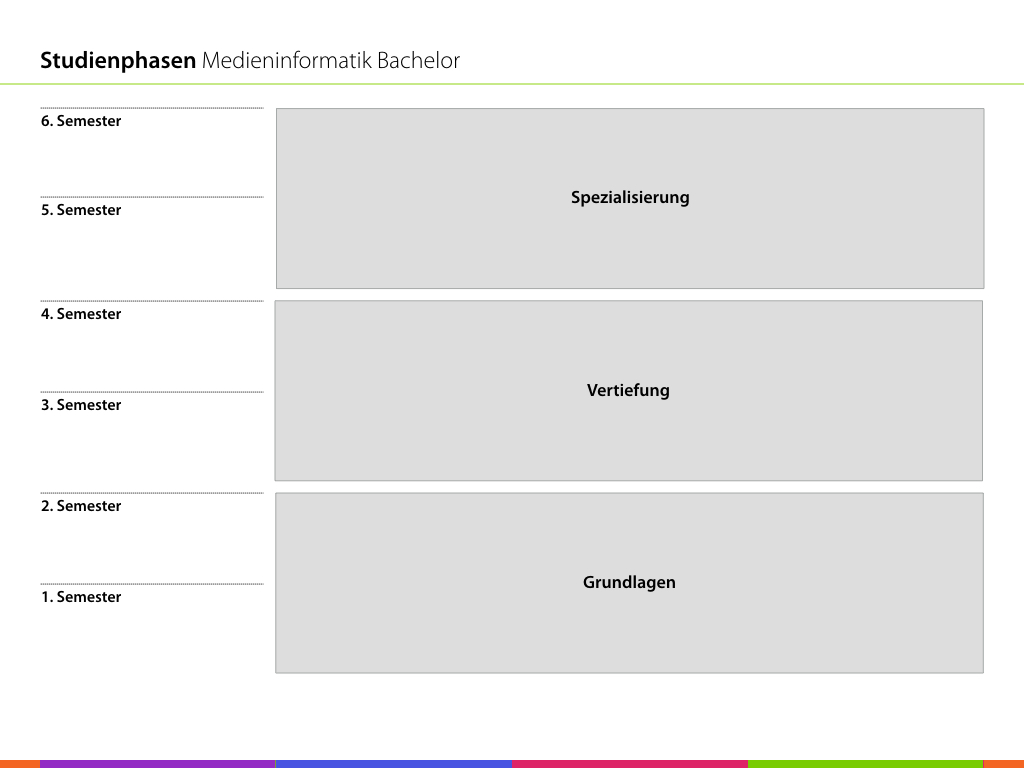
\includegraphics{../anhaenge/bilder/ba-studienphasen.001.jpeg}\{:class=``img-responsive''\}
\emph{Bild 1: Studienphasen des Bachelorstudiengangs Medieninformatik}

\chapter{Veränderungen des
Studienprogramms}\label{veruxe4nderungen-des-studienprogramms}

\section{Veränderungen des
Bachelorstudienprogramms}\label{veruxe4nderungen-des-bachelorstudienprogramms}

Die im Folgenden dargestellten geplanten Veränderungen des
Bachelorstudienprogramms dienen zur Beseitigung erkannter Schwächen

\begin{itemize}
\tightlist
\item
  Verbesserung der Studierbarkeit und Verringerung der Studiendauer
  (Überschreitung der Regelstudienzeiten)
\item
  Größere praxisund projektorientierte Ausrichtung
\item
  Größere internationale Ausrichtung
\item
  Defragmentierung von Modulen und projektorientierten Praxisanteilen
  und zur Maßnahmenbildung im Rahmen der Ziele der Hochschul- und
  Fakultätsentwicklungspläne
\item
  Integrierte Programme und Maßnahmen, die sich gegenseitig verstärken
\item
  Profil stärken, Alleinstellungsmerkmale entwickeln und Attraktivität
  erhöhen
\item
  Internationalität stärken
\item
  Übergang ins Berufsleben und Kooperation mit Unternehmen durch
  stärkere Projektorientierung verbessern
\end{itemize}

\section{Geplante Veränderungen
Bachelor}\label{geplante-veruxe4nderungen-bachelor}

Geplant ist eine bessere Berücksichtigung der Lernaufwände in den
einzelnen Modulen. Nach einer Überprüfung der Aufwände wurden in vielen
Modulen bereits Anpassungen der Lehrformate, des Projektanteils und der
Prüfungsformen vorgenommen. Veranstaltungen aus einem Themenbereich
werden zukünftig möglichst in einem Semester zusammengefasst um damit
häufige Perspektivund Themenwechsel zu vermeiden und Praxisanteile
zusammenfassen zu können. Damit kann wird auch eine sinnvollere
Staffelung der projektbasierten Praxisanteile möglich, so dass die
Studierenden besser auf das 10-Creditpoint Projekt im fünften Semester
vorbereitet sind. Dieses Projekt kann zukünftig thematisch stärker durch
die Studierenden bestimmt werden. Hiermit ist zum einen eine bessere
Möglichkeit zur Vertiefung gegeben und zum anderen kann dadurch schon
der Weg ins Abschluss Semester thematisch vorbereitet werden. Über neue
Wahlmöglichkeiten, können die Studierenden, entsprechend ihrer Neigung,
zukünftig besser eigene Qualifizierungsschwerpunkte setzen.

Das im fünften Semester fast ausschließlich projektbasierte Studium
eröffnet zudem die Möglichkeit, ein Semester im Ausland zu verbringen,
dort zu arbeiten oder an einer ausländischen Hochschule Projekte zu
bearbeiten. Insofern wird dem zunehmenden Anspruch an eine größere
internationale Ausrichtung des Studiengangs auf flexible Art und Weise
entsprochen.

Einige inhaltliche Veränderungen am Zuschnitt der Module dienen der
stärkeren Orientierung auf das Berufsfeld der Absolventen. Insbesondere
interkulturelle Teamkompetenz, Projektmanagement, soziale Kompetenz und
auch die Vorbereitung auf Führungsaufgaben wird verstärkt. Dies soll vor
allem durch Integration der entsprechenden Wissensmodule in die
fachlichen Module erreicht werden.

\section{Synergien innerhalb der Informatik Bachelor
Studiengänge}\label{synergien-innerhalb-der-informatik-bachelor-studienguxe4nge}

Im Zuge der Vorbesprechungen zur Reakkreditierung wurden und werden
derzeit Gespräche mit den Studiengangsmanagern aller Informatik
Studiengänge der Fakultät 10 und im Institut für Informatik geführt. Das
Ziel ist, den organisatorischen Rahmen der Bachelor Studiengänge
möglichst gleich zu gestalten um nach wie vor innerhalb einer
gemeinsamen Prüfungsordnung agieren zu können und Synergien weiterhin
nutzbar zu machen.

\section{Veränderungen des
Masterstudienprogramms}\label{veruxe4nderungen-des-masterstudienprogramms}

Die im Folgenden dargestellten geplanten Veränderungen des
Masterstudienprogramms dienen zur Beseitigung erkannter Schwächen

\begin{itemize}
\tightlist
\item
  Fehlende Profilschärfung und Praxisbezug
\item
  Geringer Anteil an projektbasierter Lehre
\item
  Geringe internationale Ausrichtung
\end{itemize}

und zur Maßnahmenbildung im Rahmen der Ziele der Hochschul- und
Fakultätsentwicklungspläne wie sie bereits oben beim
Bachelorstudienprogramm dargestellt wurden.

\section{Geplante Veränderungen
Master}\label{geplante-veruxe4nderungen-master}

Der Studiengang erhält Vertiefungsrichtungen. Es werden Wahlkataloge im
Umfang von 24 Creditpoints angeboten. Je nach Neigung kann durch
entsprechende Auswahl von Modulen ein spezieller Teilbereich der
Medieninformatik studiert werden. Zugleich ergeben sich weitere
Synergieeffekte mit dem auch vom Institut für Informatik angebotenen
Master „Informatik`` mit den beiden Studienrichtungen „Software
Engineering`` und „Information Systems``. Diese Maßnahme wirkt auch
langfristig hinsichtlich des zu erwartenden Anstiegs der
Bewerbernachfrage für dieses Studienangebot aus. Zugleich werden die
Studierenden besser auf die Aufgaben in der Praxis vorbereitet.

Der Projektanteil wird von 10 Creditpoints auf 36 Creditpoints erhöht
und auf alle Studiensemester verteilt, sodass der Übergang ins
Berufsleben und die Kooperation mit Unternehmen verbessert werden
können. Zu der praktischen Projektarbeit gesellen sich jeweils
fachlicher Anteile. z.B. in Form von seminaristischenoder
Vorlesungsanteilen. Die Mitarbeit der Studierenden in Projekten trägt
überdies zum Ausbau der Forschungsaktivitäten der Fakultät bei. Außerdem
bietet sich das dritte Semester mit seiner fast ausschließlichen
Projektorientierung für einen Forschungsaufenthalt im Ausland an.

Der Anteil der Pflicht-Lehrveranstaltungen sinkt von 75 Creditpoints auf
18 Creditpoints. Diese werden auf das erste und zweite Semester
konzentriert und teilweise in Form von Wahlkatalogen angeboten. Das
Verhältnis von Präsenzanteil zu Arbeitsaufwand wird reduziert, sodass
für die Studierenden mehr Zeit für Ausarbeitungen, Referate und
Literaturstudium bleibt und einer Verschulung des Masterstudiums
entgegen wirkt. Zu diesem Zweck werden alle Module mit 6 Creditpoints
statt bisher mit 5 Creditpoints ausgestattet.

Einige inhaltliche Veränderungen am Zuschnitt der Module dienen der
stärkeren Orientierung auf das Berufsfeld der Masterabsolventen.
Insbesondere die Vorbereitung auf Führungsaufgaben wird durch ein neu
eingeführtes Pflichtmodul von 6 Creditpoints deutlich verstärkt. Die
geplanten Veränderungen stehen in völliger Übereinstimmung mit den
Plänen der Hochschule und der Fakultät und sind geeignet, die Erreichung
der entsprechenden Ziele nachhaltig zu unterstützen.

\section{Synergien innerhalb der Informatik Master
Studiengänge}\label{synergien-innerhalb-der-informatik-master-studienguxe4nge}

Auch hier wurden intensive Gespräche mit den Studiengangsmanagern aller
Informatik Studiengänge der Fakultät 10 und im Institut für Informatik
geführt. Zwar lässt sich in den Masterstudiengänge wahrscheinlich keine
gemeinsame Prüfungsordnung installieren, dennoch wurden einige Maßnahmen
verabschiedet, um mehr Synergien zwischen Studienangeboten nutzbar zu
machen. Vor allem die einheitliche Modulgröße von 6 Creditpoints und der
einheitliche Zuschnitt der Projekte erhöhen das synergetische Potential
signifikant.

\section{Übergreifende
Ausrichtung}\label{uxfcbergreifende-ausrichtung}

Bewusst wird in den Studiengängen der Medieninformatik auf eine
Annäherung an das medientechnikbezogene Angebot der Fakultät 7 vermieden
und stattdessen eine Profilierung und Abgrenzung durch die Fokussierung
auf die Informatik-Anteile und die verstärkte Projektorientierung, im
Master auch höhere Forschungsorientierung, erreicht.

\chapter{Vereinbarkeit mit der
Fakultätsplanung}\label{vereinbarkeit-mit-der-fakultuxe4tsplanung}

Die Vereinbarkeit der Reakkreditierung und Fortführung der beiden
Studiengänge kann nur im Rahmen der insgesamt von der Lehreinheit
Informatik angebotenen Bachelorund Master-Studiengänge begründet werden.
Im Anhang D findet sich die auf einer Zusammenstellung der von der
Lehreinheit angebotenen Module und den Kapazitäts-Rahmendaten basierende
aktuelle Kapazitätsberechnung der Lehreinheit Informatik. Lehrimporte
und Lehrexporte sind dabei ebenso berücksichtigt wie die erteilten
Lehraufträge. Es handelt sich dabei um eine Fortschreibung der im
Wintersemester 11/12 anlässlich der Akkreditierung der weiteren von der
Lehreinheit erbrachten BA/MA-Studiengänge aufgestellten
Kapazitätsberechnung hinsichtlich der seitdem vorgenommenen
unwesentlichen Änderungen der Module und Studienverlaufspläne sowie der
aktuellen Studierendenzahlen. Eine auf der aktuellen Kapazitätslage
fußende Berechnung wird nachgereicht.

Der Vergleich der Kennzahlen in Anhang D zeigt, dass die Kapazitäten des
Instituts für Informatik gut den Erfordernissen der angebotenen
Studiengänge entsprechen. Die verhältnismäßige Aufteilung zwischen
Bachelor und Master errechnet sich als 1/5 zu 4/5 oder prozentual als
18,2\% zu 81,8\%. Dabei sind zu 10\% bzw. 5\% Leistungen von
Lehrbeauftragen berücksichtigt, wie sie auch bisher aufgebracht werden.
Synergie- effekte zwischen den Bachelorstudiengängen der Informatik
sorgen dafür, dass wesentliche Pflichtveranstaltungen in gewohntem Maß
durchgeführt werden können und genügend Kapazität für
studiengangsspezifische Veranstaltungen sowohl im Bachelor als auch im
Master verbleibt. Insgesamt stellt sich die kapazitive Situation des
Instituts für Informatik den zukünftigen Erfordernissen entsprechend mit
102,8\% als Verhältnis zwischen planmäßigem und anvisiertem Potential
als angemessen dar.

\chapter{Zusammenfassung}\label{zusammenfassung}

Zusammengefasst stellen sich die beiden vom Institut für Informatik der
Fakultät 10 getragenen Studiengänge Medieninformatik Bachelor und
Medieninformatik Master gemäß der vorliegenden Daten und Erfahrungen als
ein, sowohl hinsichtlich der Nachfrage der Studierenden und des
Lehr-Portfolios der Fakultät 10 und auch hinsichtlich des Bedarfs der
regionalen und überregionalen Industrie, hervorragend aufgestelltes und
etabliertes Lehrangebot der TH Köln dar.

\chapter{Studierbarkeit}\label{studierbarkeit}

\chapter{Prüfungssystem}\label{pruxfcfungssystem}

\chapter{Studiengangsbezogene
Kooperationen}\label{studiengangsbezogene-kooperationen}

\chapter{Ausstattung}\label{ausstattung}

\section{Verleih}\label{verleih}

\begin{itemize}
\item
  12 x Audiovisuelle Produktionssets, bestehend aus jeweils
\item
  P2 Panasonic HD Kamera
\item
  Sachtler Kamerastativ

  \begin{itemize}
  \tightlist
  \item
    Sennheiser MKH 416 Richtmikrofon
  \item
    2 Kanal Audiomischer
  \item
    Tonangel
  \item
    Diverse Verbindungskabel und Taschen
  \end{itemize}
\item
  4 x kompakte Panasonic HD Kameras
\item
  1 x Canon EOS 5D Mark III mit folgenden Objektiven:
\item
  Canon Fisheye Zoom Lens EF 8-15mm 1:4 L USM
\item
  Canon Zoom Lens EF 24-70mm 1:4 L IS USM
\item
  Canon Lens EF 85mm 1:1,2 L II USM
\item
  1 x GoPro Hero 3 Black Edition
\item
  1 x DJI Ozmo Gimbal Kamera
\item
  9 x Lichtset, bestehend aus jeweils
\item
  3 x 750 W ARRI Scheinwerfer
\item
  3 x Stative
\item
  1 x Koffer
\item
  Diverses Zubehör für Licht, Ton und Video:
\item
  Reflektoren
\item
  Stative
\item
  Monitore
\item
  Speichermedien
\item
  Reflektoren
\item
  Smartphones und Tablets
\item
  1 x Nexus 5
\item
  2 x Nexus 9
\item
  1 x iPad Pro 13'' mit Apple Pencil
\end{itemize}

\section{Nachbearbeitung}\label{nachbearbeitung}

\begin{itemize}
\item
  5 x Mac Pro stationär, mit Adobe Production Suite CS 6
\item
  12 x iMac mobil, mit Adobe Production Suite CS 6
\item
  1 x Tonkabine mit folgenden Equipment
\item
  Neumann Großmembranmikrofon mit Poppschutz
\item
  Mac Pro mit Logic X zur Aufnahmen und Nachbearbeitung
\item
  Mackie 1402 Tonmischpult
\end{itemize}

\section{Studio}\label{studio}

\begin{itemize}
\tightlist
\item
  Greenbox mit festmontierter und variabler Beleuchtung
\item
  Bildmischer Panasonic AV-HS400A
\item
  Audiomischer Behringer AB1222FX-Pro
\item
  Mac Pro mit Adobe Production Suite CS 6 zur Digitalisierung und
  Nachbearbeitung der Studioproduktionen
\end{itemize}

\section{Lehrende in der
Medieninformatik}\label{lehrende-in-der-medieninformatik}

\subsection{Prof.~Dr.~Thomas
Bartz-Beielstein}\label{prof.dr.thomas-bartz-beielstein}

\begin{itemize}
\tightlist
\item
  Forschungsschwerpunkt CIplus
\item
  Web: https://www.th-koeln.de/personen/thomas.bartz-beielstein/
\item
  Lehrgebiete:

  \begin{itemize}
  \tightlist
  \item
    Angewandte Mathematik Simulation und Optimierung~
  \item
    Computational Intelligence Evolutionäre Algorithmen
  \end{itemize}
\end{itemize}

\textbf{Bente, Stefan}

https://www.th-koeln.de/personen/stefan.bente/

Lehrgebiete

\begin{itemize}
\tightlist
\item
  Softwaretechnik Softwarearchitektur
\item
  Anforderungsmanagement
\end{itemize}

\textbf{Bertelsmeier, Birgit}

https://www.th-koeln.de/personen/birgit.bertelsmeier/

Lehrgebiete

\begin{itemize}
\tightlist
\item
  Datenbank- und Informationssysteme RDBMS bis NoSQL
\end{itemize}

\textbf{Böhmer, Matthias}

https://www.th-koeln.de/personen/matthias.boehmer/

Lehrgebiete

\begin{itemize}
\tightlist
\item
  Mobile und Verteilte Architekturen
\end{itemize}

\textbf{Eisemann, Martin}

https://www.th-koeln.de/personen/martin.eisemann/

Lehrgebiete

\begin{itemize}
\tightlist
\item
  Computergrafik Realistische und Interaktive Bildsynthese, Bildbasierte
  Computergraphik, Visual Analytics, Gaming Technologies
\item
  Theoretische Informatik Grundlagenvorlesungen im Bachelor
\end{itemize}

\textbf{Faeskorn-Woyke, Heide}

https://www.th-koeln.de/personen/heide.faeskorn-woyke/

Lehrgebiete

\begin{itemize}
\tightlist
\item
  Datenbanken und Informationssysteme
\end{itemize}

\textbf{Fischer, Kristian}

https://www.th-koeln.de/personen/kristian.fischer/

Lehrgebiete

\begin{itemize}
\tightlist
\item
  Web-basierte Anwendungen und verteilte Systeme
\end{itemize}

\textbf{Giannakopoulos, Fotios}

https://www.th-koeln.de/personen/fotios.giannakopoulos/

Lehrgebiete

\begin{itemize}
\tightlist
\item
  \textbf{{[}hier fehlt noch Inhalt{]}}
\end{itemize}

\textbf{Günther, Holger}

https://www.th-koeln.de/personen/holger.guenther/

Lehrgebiete

\begin{itemize}
\tightlist
\item
  \textbf{{[}hier fehlt noch Inhalt{]}}
\end{itemize}

\textbf{Hartmann, Gerhard}

https://www.th-koeln.de/personen/gerhard.hartmann/

Lehrgebiete

\begin{itemize}
\tightlist
\item
  Mensch-Computer Interaktion
\item
  Entwicklungsprojekt interaktive Systeme
\item
  Interaction Design
\item
  Naturwissenschaftliche Grundlagen Digitaler Medien
\item
  Research Methods in Human-Computer Interaction
\item
  Design Methodologies
\end{itemize}

\textbf{Jochum, Friedbert}

https://www.th-koeln.de/personen/friedbert.jochum/

Lehrgebiete

\begin{itemize}
\tightlist
\item
  \textbf{{[}hier fehlt noch Inhalt{]}}
\end{itemize}

\textbf{Karsch, Stefan}

https://www.th-koeln.de/personen/stefan.karsch/

Lehrgebiete

\begin{itemize}
\tightlist
\item
  \textbf{{[}hier fehlt noch Inhalt{]}}
\end{itemize}

\textbf{Klocke, Heinrich}

https://www.th-koeln.de/personen/heinrich.klocke/

Lehrgebiete

\begin{itemize}
\tightlist
\item
  Mensch-Computer Interaktion Usability Engineering und kognitive
  Psychologie
\item
  Algorithmik
\item
  Künstliche Intelligenz Logische Agenten
\end{itemize}

\textbf{Knittel, Friedrich}

https://www.th-koeln.de/personen/friedrich.knittel/

Lehrgebiete

\begin{itemize}
\tightlist
\item
  \textbf{{[}hier fehlt noch Inhalt{]}}
\end{itemize}

\textbf{Koch, Heribert}

https://www.th-koeln.de/personen/heribert.koch/

Lehrgebiete

\begin{itemize}
\tightlist
\item
  \textbf{{[}hier fehlt noch Inhalt{]}}
\end{itemize}

\textbf{Köhler, Lutz}

https://www.th-koeln.de/personen/lutz.koehler/

Lehrgebiete

\begin{itemize}
\tightlist
\item
  \textbf{{[}hier fehlt noch Inhalt{]}}
\end{itemize}

\textbf{Kohls, Christian}

https://www.th-koeln.de/personen/christian.kohls/

Lehrgebiete

\begin{itemize}
\tightlist
\item
  \textbf{{[}hier fehlt noch Inhalt{]}}
\end{itemize}

\textbf{Konen, Wolfgang}

https://www.th-koeln.de/personen/wolfgang.konen/

Lehrgebiete

\begin{itemize}
\tightlist
\item
  Mathematik
\item
  Data Mining
\end{itemize}

\textbf{Kornacher, Hans Hermann}

https://www.th-koeln.de/personen/hans.kornacher/

Lehrgebiete

\begin{itemize}
\tightlist
\item
  Medientechnik und -produktion
\item
  Digitale Animation und Visual Effects in der Film- und
  Fernsehproduktion
\end{itemize}

\textbf{Naujoks, Boris}

https://www.th-koeln.de/personen/boris.naujoks/

Lehrgebiete

\begin{itemize}
\tightlist
\item
  Angewandte Mathematik Grundlagenveranstaltungen Informatik und
  Ingenieure
\end{itemize}

\textbf{Noss, Christian}

https://www.th-koeln.de/personen/christian.noss/

Lehrgebiete

\begin{itemize}
\tightlist
\item
  Kommunikationsdesign
\item
  Web-basierte Anwendungen
\end{itemize}

\textbf{Stahl, Hans Ludwig}

https://www.th-koeln.de/personen/hans.stahl/

Lehrgebiete

\begin{itemize}
\tightlist
\item
  Theoretische Informatik und Technische Informatik
\item
  Kommunikationstechnik und Netze
\item
  Mobile IT Security
\item
  IT Compliance and Risk Management Informatik
\end{itemize}

\textbf{Victor, Frank}

https://www.th-koeln.de/personen/frank.victor/

Lehrgebiete

\begin{itemize}
\tightlist
\item
  \textbf{{[}hier fehlt noch Inhalt{]}}
\end{itemize}

\textbf{Westenberger, Hartmut}

https://www.th-koeln.de/personen/hartmut.westenberger/

Lehrgebiete

\begin{itemize}
\tightlist
\item
  Informatik Betriebliche Anwendungssysteme
\end{itemize}

\textbf{Winter, Mario}

https://www.th-koeln.de/personen/mario.winter/

Lehrgebiete

\begin{itemize}
\tightlist
\item
  Softwareentwicklung und Projektmanagement in Medienprojekten
\item
  Modellbasierte Entwicklungsmethoden und Qualitätssicherung
\end{itemize}

\chapter{Transparenz und
Dokumentation}\label{transparenz-und-dokumentation}

\chapter{Qualitätssicherung und
Weiterentwicklung}\label{qualituxe4tssicherung-und-weiterentwicklung}

Die TH Köln betrachtet Gleichstellung und Chancengleichheit der
Geschlechter als Querschnittsaufgaben. Dabei wird Gleichstellung als
integrierter Bestandteil von Lehre und Forschung verstanden, auf die
Vereinbarkeit von Studium und Familie beziehungsweise Beruf und Familie
geachtet sowie für eine ausgewogene Beteiligung von Männern und Frauen
an den Entscheidungsstrukturen in Lehre, Forschung und Verwaltung
gesorgt. Darüber hinaus wird der Anteil der Frauen bei den Professuren,
Mitarbeiterstellen und den Studierenden in denjenigen Fächern, in denen
sie unterrepräsentiert sind, kontinuierlich erhöht.

Es wird die Aufstellung und Einhaltung der Frauenförderpläne
kontrolliert. Des Weiteren werden bei einem ``Girl's Day'' spezielle
Veranstaltungen für interessierte Frauen bezüglich der
Informatikstudiengänge angeboten. Alle Konzepte und Maßnahmen für
Geschlechtergerechtigkeit und Chancengleichheit finden auf die zu
akkreditierenden Studiengänge Anwendung.

Fernerhin hat die TH Köln das Audit familiengerechte
Hochschule\footnote{https://www.th-koeln.de/hochschule/familienfreundlichkeit\_3759.php}
der berufundfamilie gemeinnützigen GmbH erfolgreich durchgeführt. Im
Rahmen der Auditierung wurden der Bestand familienorientierter Maßnahmen
begutachtet und weiterführende Zielvorgaben zur Verwirklichung
familiengerechter Studienbedingungen sowie einer familienbewussten
Personalpolitik definiert. Die Hochschule ist in 2015 erfolgreich
re-auditiert worden.

\section{Konzepte zur Förderung der
Chancengleichheit}\label{konzepte-zur-fuxf6rderung-der-chancengleichheit}

Die Konzepte zur Förderung der Chancengleichheit gelten insbesondere für
Studierende in besonderen Lebenslagen (z.B. Studierende mit Kind), für
Studierende mit Beeinträchtigung oder für Studierende mit spezifischem
sozialem Hintergrund.

Die TH Köln versteht sich als familiengerechte Hochschule und bietet
verschiedene Beratungsangebote und Serviceleistungen für studierende
Eltern an, um die Vereinbarkeit von Studium/Beruf und Familie besser zu
ermöglichen. Im Herbst 2009 wurde das Programm ``Educational Diversity''
der TH Köln aufgesetzt. Die Grundidee von Educational Diversity ist die
Umsetzung einer gelebten, die Unterschiedlichkeit der Studierenden als
kreatives Potenzial begreifenden Lehr- und Lerncommunity. Alle Akteure
stehen im direkten Kontakt miteinander und werden durch eine webbasierte
Lehr- und Lerncommunity unterstützt.

Das Programm „Educational Diversity``\footnote{https://www.th-koeln.de/hochschule/educational-diversity\_5710.php}
der TH Köln hat zum Ziel, die Verschiedenartigkeit der Studierenden zu
erkennen und durch hochschuldidaktische Differenzierung das Potenzial
jedes/jeder einzelnen Studierenden optimal zu fördern. Auch die
Dozent*innen der Informatikstudiengänge beteiligen sich an diesen
Programmen.

\section{Konzept der Hochschule für Chancengleichheit und Studierende
in besonderen
Lebenslagen}\label{konzept-der-hochschule-fuxfcr-chancengleichheit-und-studierende-in-besonderen-lebenslagen}

Für die Umsetzung der Chancengleichheit von Männern und Frauen hat die
Hochschule in ihrem Entwicklungsplan vier Ziele benannt: 1. Die
Ermöglichung einer geschlechtsunabhängigen Studienfachwahl für
Schülerinnen und Schüler. 2. Die Erhöhung des Frauenanteils bei den
wissenschaftlichen Beschäftigten der TH Köln, insbesondere bei den
Professorinnen, wissenschaftlichen Mitarbeiterinnen und
Lehrbeauftragten. 3. Die Verbesserung der Vereinbarkeit von Studium bzw.
Beruf und Familie. 4. Die Umsetzung bzw. Unterstützung genderbezogener
Projekte in Lehre und Forschung.

Die Umsetzung dieser Ziele und die Einbettung in die bestehenden
Handlungsfelder der Hochschule werden in der amtlichen
Mitteilung\footnote{http://www.fh-koeln.de/mam/downloads/deutsch/hochschule/profil/gleichstellung/gleichstellungskonzept.pdf}
näher erläutert. Der TH Köln ist es ein besonderes Anliegen, mit den
umgesetzten Maßnahmen die Selbstverständlichkeit von Beruf und Familie
bzw. Studium und Familie zu unterstreichen und damit eine
Kulturveränderung innerhalb der Hochschule zu bewirken, denn damit
werden indirekt Karrierehemmnisse von Frauen abgebaut.

\begin{verbatim}
    Aktueller Bearbeiter: -
    Bearbeiterhistorie: Christian Noss
    Date: 17.02.2017
    Comment: alles von Websience geklaut … danke!
    Status: fertig, review erfolrderlich
    Reviewed von: -
\end{verbatim}

\chapter{Backlog}\label{backlog}

Folgende Themen sollten noch adressiert werden:

\begin{itemize}
\tightlist
\item
  Entwicklung der Medieninformatik insgesamt
\item
  Veranstaltungen und Formate: Showcase, Kontaktbörse, Filmfest,
  Website, Youtube Kanal, Twitter, Facebook
\item
  Top 5 Studiengang laut
  https://www.studycheck.de/studium/medieninformatik
\item
  auf welcher Basis wurde konzipiert: GI Paper, Gruppe Medieninformatik
  der GI
\item
  Toolchain
\item
  Abgleich mit Fakultätsentwicklungsplan?
\end{itemize}

\chapter{Inhalte aus dem Antrag, die übrig geblieben
sind}\label{inhalte-aus-dem-antrag-die-uxfcbrig-geblieben-sind}

\begin{enumerate}
\def\labelenumi{\arabic{enumi}.}
\tightlist
\item
  Es kommt zu einer besseren Berücksichtigung der Lernaufwände der
  Studierenden in den einzelnen Modulen. Nach einer Überprüfung der
  Aufwände wurden in vielen Modulen bereits Anpassungen der Lehrformate,
  des Projektanteils und der Prüfungsformen vorgenommen. Die Anzahl der
  Veranstaltungen wird reduziert und die Fächer mit höherem Lernaufwand
  und höherem Schwierigkeitsgrad werden im Studienverlaufsplan neu
  angeordnet, um den Aufwand gleichmäßiger über das Studium zu
  verteilen.
\item
  Eine Neusortierung und Zuordnung der Module zu den Semestern sorgt für
  eine gleichmäßigere Verteilung der Lernaufwände auf die Semester. Die
  Prüfungsanteile wurden hierbei entsprechend berücksichtigt. So wurden
  beispielsweise vergleichsweise ``schwerere und aufwändige'' Module aus
  dem bisher überlasteten 3. Semester auf andere Semester verteilt.
\end{enumerate}

Die Praxisorientierung wird durch Projekte innerhalb der Module und
expliziten Projektmodulen erreicht. Der Umfang der Projektanteile wird
über die Semester langsam erhöht, so dass im Studienverlauf komplexere
Projekte mit verschiedenen fachlichen Perspektiven bearbeitet werden
können.

\begin{enumerate}
\def\labelenumi{\arabic{enumi}.}
\setcounter{enumi}{2}
\tightlist
\item
  Das im fünften Semester sehr stark projektbasierte Studium eröffnet
  zudem die Möglichkeit, ein Semester im Ausland zu verbringen, dort zu
  arbeiten oder an einer ausländischen Hochschule Projekte zu
  bearbeiten. Insofern wird dem zunehmenden Anspruch an eine größere
  internationale Ausrichtung des Studiengangs auf flexible Art und Weise
  entsprochen.
\end{enumerate}

Die Studierenden haben die Möglichkeit das Studium, ihren Neigungen
entsprechend, zu vertiefen. Das Curriculum sieht dafür, neben den
bereits erwähnten Vertiefungsmodulen im vierten Semester, ein großes
Projekt im fünften Semester, sowie das Praxisprojekt und die
Bachelorarbeit im Abschlusssemester vor.

\begin{enumerate}
\def\labelenumi{\arabic{enumi}.}
\setcounter{enumi}{3}
\tightlist
\item
  Einige inhaltliche Veränderungen am Zuschnitt der Module dienen der
  stärkeren Orientierung auf das Berufsfeld der Absolventen.
  Insbesondere interkulturelle Teamkompetenz, Projektmanagement, soziale
  Kompetenz und auch die Vorbereitung auf Führungsaufgaben wird
  verstärkt. Dies soll vor allem durch Integration der entsprechenden
  Wissensmodule in die fachlichen Module erreicht werden.
\end{enumerate}

Als Kernfächer der Medieninformatik werden die Module ``Einführung in
die Medieninformatik'', ``Mensch-Computer-Interaktion'',
``Screendesign'', ``Web Fundamentals'', ``Audiovisuelles Medienprojekt''
und ``Medienrecht, Medien \& Gesellschaft'' angeboten. Im vierten
Semester kann eine von drei Fachvertiefungen gewählt werden. Hier stehen
die Module ``Visual Computing'', ``Social Computing'' und ``Web
Development'' zur Wahl.

Geplant ist eine bessere Berücksichtigung der Lernaufwände in den
einzelnen Modulen. Nach einer Überprüfung der Aufwände wurden in vielen
Modulen bereits Anpassungen der Lehrformate, des Projektanteils und der
Prüfungsformen vorgenommen. Veranstaltungen aus einem Themenbereich
werden zukünftig möglichst in einem Semester zusammengefasst um damit
häufige Perspektiv- und Themenwechsel zu vermeiden und Praxisanteile
zusammenfassen zu können. Damit wird auch eine sinnvollere Staffelung
der projektbasierten Praxisanteile möglich, so dass die Studierenden
besser auf das 10-CP Projekt im fünften Semester vorbereitet sind.
Dieses Projekt kann zukünftig thematisch stärker durch die Studierenden
bestimmt werden. Hiermit ist zum einen eine bessere Möglichkeit zur
Vertiefung gegeben und zum anderen kann dadurch schon der Weg ins
Abschlusssemester thematisch vorbereitet werden. über neue
Wahlmöglichkeiten, können die Studierenden, entsprechend ihrer Neigung,
zukünftig besser eigene Qualifizierungsvertiefungen setzen.

Das im fünften Semester fast ausschließlich projektbasierte Studium
eröffnet zudem die Möglichkeit, ein Semester im Ausland zu verbringen,
dort zu arbeiten oder an einer ausländischen Hochschule Projekte zu
bearbeiten. Insofern wird dem zunehmenden Anspruch an eine größere
internationale Ausrichtung des Studiengangs auf flexible Art und Weise
entsprochen.

Einige inhaltliche Veränderungen am Zuschnitt der Module dienen der
stärkeren Orientierung auf das Berufsfeld der Absolventen.
